\documentclass[a4paper,12pt]{report}
%%%%%%%%%%%%%%%%%%%%%%%%%%%%%%%%%%%%%%%%%%%%%%%%%%%%%%%%%%%%%%%%%%%%%%%%%
%%%%%% Definizioni:
\def\titolotesi{Realizzazione di un'interfaccia per l'interazione uomo-macchina basato su head-tracking} % INSERIRE TIOLO DELLA TESI
\def\laureando{Michele Matriciani}       % INSERTIRE NOME COGNOME LAUREANDO
\def\annoaccademico{2012--2013}    % INSERIRE ANNO ACCADEMICO
\def\dedica{Dedica...}      % INSERIRE DEDICA


%%%%%% File previsti in input:
%% introduzione.tex    (deve contenere solo il testo, senza \chapter{})
%% capitolo1.tex       (deve iniziare con \chapter{titolo capitolo})
%% capitolo2.tex                           "
%% capitolo3.tex                           "
%% capitolo4.tex                           "
%% conclusioni.tex     (deve contenere solo il testo, senza \chapter{})
%% appendice.tex       (deve contenere solo il testo, senza \chapter{})
%%%%%%%%%%%%%%%%%%%%%%%%%%%%%%%%%%%%%%%%%%%%%%%%%%%%%%%%%%%%%%%%%%%%%%%%%


\usepackage[utf8]{inputenc}
\usepackage[T1]{fontenc}
\usepackage[italian]{babel}
\usepackage{amsmath}
\usepackage{graphicx}
\usepackage{float}


%FOR WRITE C++ CODE
\usepackage{listings}
\usepackage{xcolor}
\definecolor{listinggray}{gray}{0.9}
\definecolor{lbcolor}{rgb}{0.9,0.9,0.9}
\lstset{
backgroundcolor=\color{lbcolor},
    tabsize=2,    
%   rulecolor=,
    language=[GNU]C++,
        basicstyle=\footnotesize,
        %upquote=true,
        aboveskip={1.5\baselineskip},
        columns=fixed,
        showstringspaces=false,
        extendedchars=false,
        breaklines=true,
        prebreak = \raisebox{0ex}[0ex][0ex]{\ensuremath{\hookleftarrow}},
        frame=single,
        %numbers=left,
        showtabs=false,
        showspaces=false,
        showstringspaces=false,
        identifierstyle=\ttfamily,
        keywordstyle=\color[rgb]{0,0,1},
%        commentstyle=\color[rgb]{0.026,0.512,0.095},
		commentstyle=\color[rgb]{0.1,0.5,0.1},
        stringstyle=\color[rgb]{0.627,0.126,0.941},
        numberstyle=\color[rgb]{0.205, 0.142, 0.73},
%        \lstdefinestyle{C++}{language=C++,style=numbers}.
}


% Title Page
\title{\begin{large}\textbf{\titolotesi}\end{large}}
\author{\laureando}

\usepackage{fancyhdr}
\fancyhf{}
%\fancyhead[RO]{\the\chaptermark}
%\[LE,RO]{\bfseries\thepage \hfil}
\usepackage{epsfig}
\pagenumbering{Roman}
%\usepackage{setspace}
\newlength\sinistra
\newlength\corpo
\newlength\pagina
\setlength {\pagina} {21cm}
\setlength {\sinistra} {1.46cm}
\setlength {\corpo} {13.5cm}
\textwidth \the\corpo
\hoffset \the\sinistra
\paperwidth \the\pagina

\linespread{1.0}


\begin{document}
\begin{titlepage}
%\maketitle
 \begin{center}
\textsc{\Large Universit\`a degli Studi di Perugia}\medskip\\

{\Large Facolt\`a di Scienze Matematiche, Fisiche e Naturali}\medskip\\

\rule{10mm}{0.01mm}\medskip\\

{\small \textsc{Corso di Laurea in Informatica}}\medskip\\

%\vspace*{12mm}

\vspace*{3mm}


\includegraphics[scale=0.35]{images/logounipg.png}

\vspace*{-2.5cm}

\Large Tesi di Laurea \par\bigskip

%\vfill

\vspace*{0.3cm}

{\large \bf \titolotesi \par}

\bigskip\bigskip\bigskip

\end{center}\par
%\vspace*{0.5cm}\large

\hspace{0.05cm}Laureando:\hspace{7.3cm}Relatori:\par

\hspace{0.0cm}\emph{\laureando}\hfill\emph{Prof.~Osvaldo Gervasi}\\
\hspace{7.8cm}\hfill\emph{Dott.~Federico Frenguelli}

\vfill

\begin{center}

\rule{40mm}{0.01mm}\\

Anno Accademico \annoaccademico

\end{center}

\end{titlepage}
\newpage
\vspace*{2.5cm}
\begin{flushright}
\begin{Large}\emph{\dedica}\end{Large}
\end{flushright}
\frenchspacing


%%%%%% Ringraziamenti (opzionale)
%
%\chapter*{Ringraziamenti}
%Voglio ringraziare ....
%%%%%%%%%%%%%%%%%%%%%%%%%%%%%%%%%



\tableofcontents
%\listoffigures



%%%% fine prologo


%%%% Inizio corpo tesi

\pagestyle{fancy}
\fancyhead[RO]{\bfseries Introduzione}
\fancyfoot[LE,RO]{\thepage \hfil}







\addcontentsline{toc}{chapter}{Introduzione}

\chapter*{Introduzione}

Da qualche anno a questa parte sono stati sviluppati e messi in commercio dispositivi per la realtà virtuale, i più famosi sono la Nintendo Wii, il Kinect della Microsoft o l'Oculus Rift sviluppato da Oculus VR. Periferiche come queste sono chiamate NUI (natural user interface); esse  sono interfacce per l'interazione con sistemi virtuali, e hanno lo scopo di aumentare la sensazione della realtà durante l'utilizzo di applicazioni virtuali come i videogiochi, permettendo all'utente di sfruttare più sensi.

Il telecomando della Wii permette, indirettamente (dato il telecomando), di utilizzare il corpo umano come dispositivo di input di comandi. Il Kinect utilizza dei sensori a infrarossi e una telecamera per rilevare il corpo umano e registrare direttamente i suoi movimenti, trasformandoli in comandi di input. L'Oculus Rift è un visore che presenta dei sensori che riconoscono l'orientamento della testa, i cui movimenti sono tradotti in rotazioni della telecamera virtuale nell'applicazione, rendendo immersiva la visione, anche grazie alla presenza di due schermi che producono un effetto tridimensionale.

Il progetto trattato in questa tesi mira ad emulare dispositivi di questo genere, utilizzando semplicemente un computer e una webcam. Esso offre un'interfaccia che, tramite la webcam, utilizza la posizione del volto dell'utente per calcolare la prospettiva con cui viene visualizzata una scena tridimensionale, con lo scopo quindi di collegare la telecamera virtuale all'utente. L'obiettivo finale è quello di generare l'illusione della presenza di profondità all'interno dello schermo e di creare, quando le condizioni sono ottimali, un effetto tridimensionale senza l'utilizzo di occhiali appositi.

Dato l'utilizzo di software open source e di dispositivi di qualità media, l'effetto generato non è paragonabile a quello che può essere prodotto da sistemi più efficienti e dedicati allo scopo, tuttavia sono stati raggiunti comunque risultati notevoli.

I software impiegati nello sviluppo del progetto sono:
\begin{itemize}
\item OpenCv, per il rilevamento del volto.
\item OpenGl, per lo studio del metodo da utilizzare e per lo sviluppo dell'applicazione.
\item Blender, per la creazione di scene 3D.
\item Ogre3D, per un miglioramento dell'applicazione in termini di grafica ed efficienza.
\end{itemize}

Nel corso di questa tesi si introdurranno i software utilizzati, sarà spiegata la teoria matematica che sta dietro alle trasformazioni utilizzate, facendo un excursus sulle tecnice adottate dalla maggior parte delle applicazioni grafiche per renderizzare a chermo una scena tridimensionale, ed infine sarà trattato il progetto sviluppato, mostrando anche le problematiche riscontrate e le possibili soluzioni.Prima di tutto però, diamo dei brevi cenni riguardanti la realtà virtuale.

\begin{figure}[htbp]
\centering
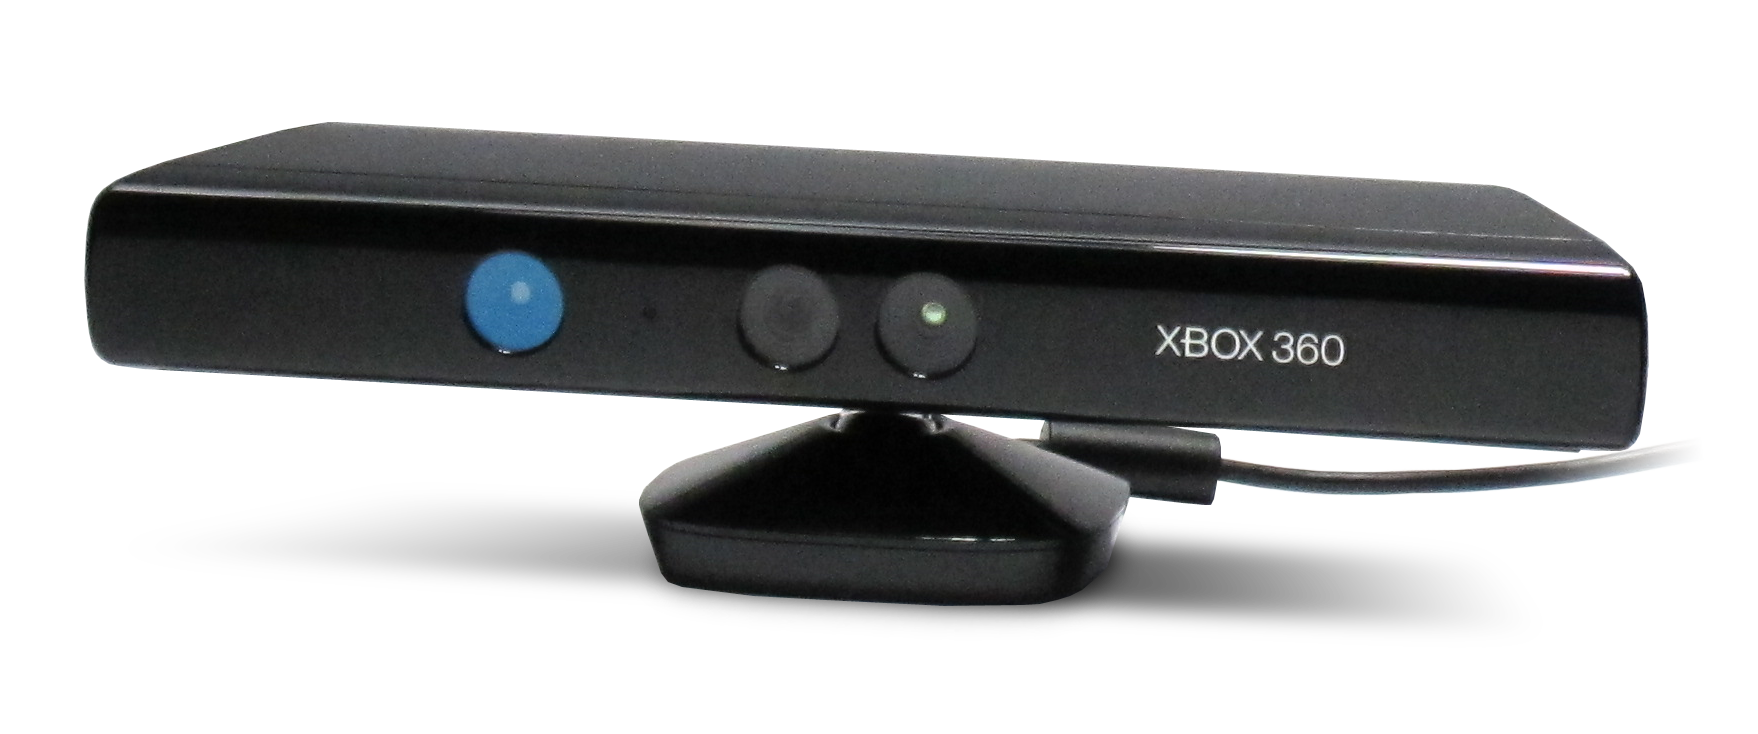
\includegraphics[width=0.4\textwidth]{images/intro/kinect.png}
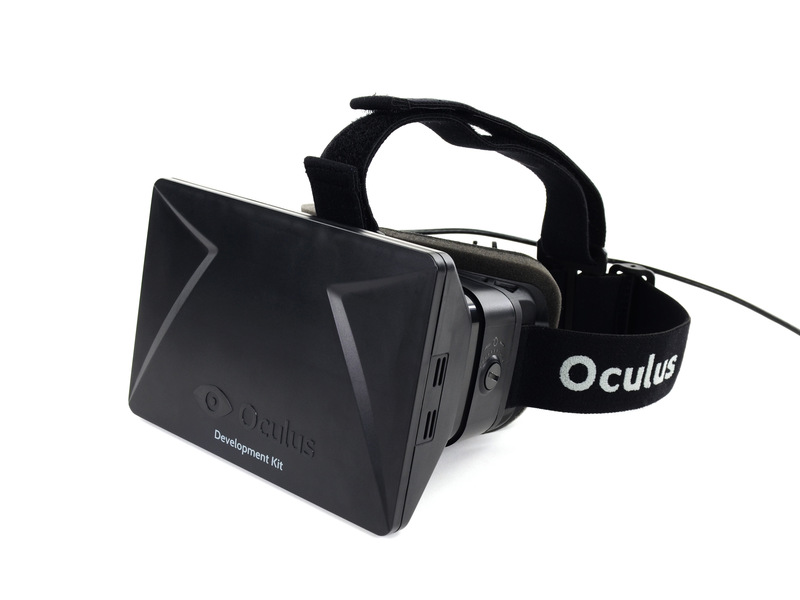
\includegraphics[width=0.4\textwidth]{images/intro/oculus-rift.jpg}
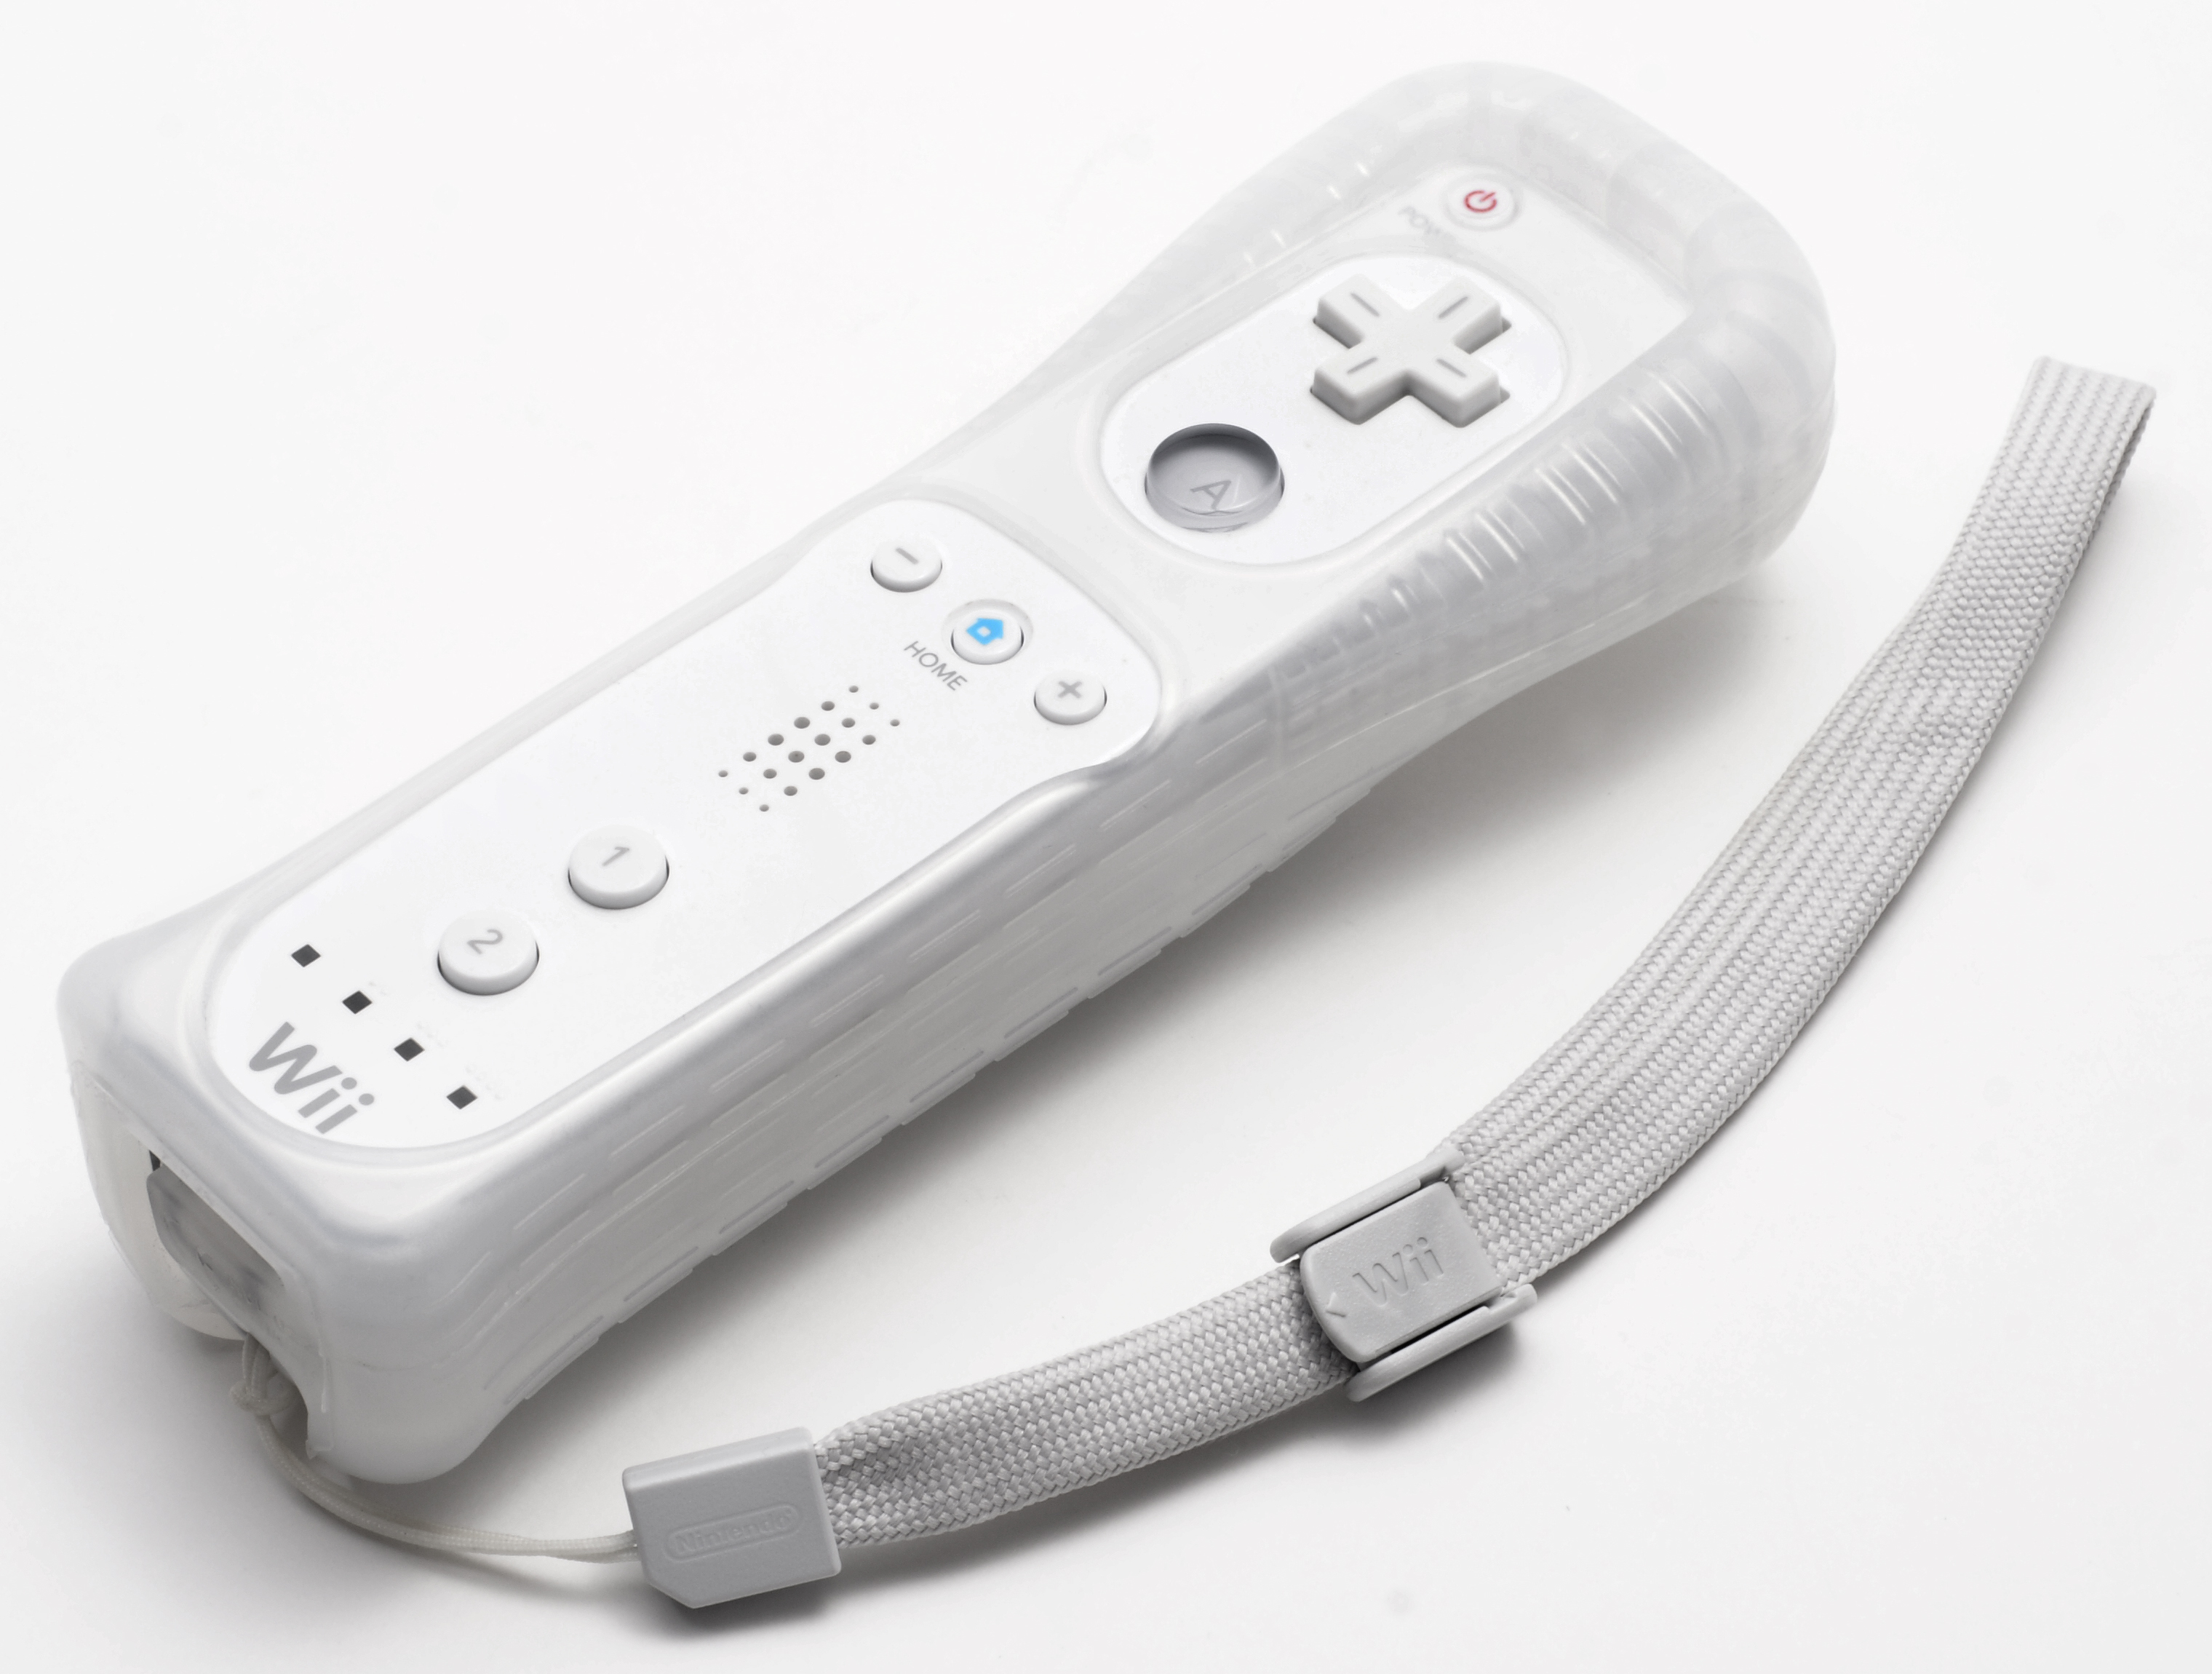
\includegraphics[width=0.4\textwidth]{images/intro/wii.jpg}
\end{figure}



\vspace{3cm}

\cleardoublepage\pagenumbering{arabic}

\chapter{Realtà virtuale}
\fancyhead[RO]{\bfseries Realtà virtuale}

Al giorno d'oggi con realtà virtuale si intende quella disciplina che ha come obiettivo simulare la realtà, cioè permettere all'utente di interagire in modo realistico e naturale con un sistema puramente virtuale. A livello teorico, un sistema ideale dovrebbe permettere all'utente un'immersione completa, con la possibilità di utilizzare tutti i sensi. Le applicazioni che fanno parte di questa categoria sono ogni tipo di simulazione virtuale creata attraverso computer, schermi, dispositivi dotati di sensori, telecamera, etc. Tra queste i videogiochi stanno prendendo piede grazie all'introduzione del 3D e di periferiche di gioco sempre più immersive.
Se, al giorno di oggi, con realtà virtuale si intende ogni forma di interazione con un sistema virtuale, nella storia essa ha avuto significati più ristretti.
 
\section{Storia}
Il termine "realtà virtuale" fu introdotto nel 1980  per indicare l'insieme dei fenomeni percettivi indotti da un'apparecchiatura cibernetica a più componenti che viene applicata a un soggetto umano.
Ad introdurre il termine fu un informatico statunitense che ha fondato la VPL Research, ricerca per i linguaggi di programmazione virtuale, ovvero Jaron Lanier.\cite{realta2}\\
Tra i dispositivi creati in questo periodo possiamo citare  il DataGlove, inventato da Thomas Zimmermann, un guantone-sensore collegabile ad un computer, oppure il display head-mounted (HMD), un visore comprendente degli schermi e dei sensori per l'orientamento, ideato da  Scott Fisher, un ricercatore della Nasa.\\
Tuttavia, in passato, quando il concetto di realtà virtuale ancora non esisteva, già erano state costruite apparecchiature che possiamo definire adatte allo scopo.\\
Uno dei primi sistemi di realtà virtuale fu sviluppato nel 1962 da Morton Heilig, il quale costruì il prototipo di un dispositivo chiamato Sensorama, che proiettava cinque film e coinvolgeva sensi quali vista,olfatto,udito e tatto, creando, come la definiva lui, una sorta di "cinema esperienza" ("Experience Theater").\\
Nel 1977 al MIT venne creato l'Aspen Movie Map, una simulazione in cui l'utente poteva camminare ed esplorare la cittadina di Aspen, in Colorado, tramite una serie di filmati che permettevano di visualizzare la maggior parte delle aree percorribili, nei limiti del possibile.

Al giorno d'oggi, uno dei dispositivi più efficienti per la realtà virtuale, tra quelli commercializzati, è l'Oculus Rift, che permette di vivere esperienze in prima persona grazie ad un visore da indossare, che possiede due schermi per avere una visione tridimensionale.
I commenti di coloro che hanno provato questo dispositivo sono positivi, in quanto la qualità della grafica e del sensore di movimento rendono l'esperienza quasi realistica.\\
Per ora ci si concentra prevalentemente sullo sviluppo di applicazioni e dispositivi destinati ad utilizzare il senso della vista. Gli altri sensi ancora sono agli esordi della realtà virtuale e stanno prendendo piede molto lentamente. Questo probabilmente perché la vista è il senso più sviluppato nell'uomo, e quindi il più adatto a percepire il realismo delle simulazioni virtuali. 

%Grazie alle tecnologie di ultima generazione e al costante miglioramento della loro efficienza, gli effetti che si possono creare sono sempre più realistici.
%La grafica oramai è giunta a livelli di qualità elevatissimi, inoltre, grazie all'aggiunta dell'effetto 3D, i risultati ottenibili sono maggiormente in grado di far immergere l'utente all'interno del mondo virtuale.\\








\chapter{Software utilizzati}
\fancyhead[RO]{\bfseries Software utilizzati}




\section{OpenCv}
Opencv (Open Source Computer Vision Library) è una libreria open source che offre funzionalità per applicazioni di computer vision.

\subsection{Storia}
Il progetto OpenCv è stato lanciato nel 1999 dalla Intel come una parte di varie iniziative volte a sviluppare applicazioni ad alta efficienza.

La versione alpha è stata rilasciata nel 2000 mentre successivamente sono state rilasciate varie versioni beta; il rilascio della versione 1.0 è avvenuto
nel 2006.

Dal 2008 il progetto è supportato dalla casa di produzione e ricerca Willow Garage, che si occupa di sviluppo di hardware e software open source per applicazioni robotiche. Nel 2009 è stata rilasciata una versione più efficiente, caratterizzata da migliori implementazioni e più funzionalità, delle quali una è la possibilità di parallelizzare il lavoro nei sistemi multi-core.

\subsection{Computer vision}

La computer vision è una disciplina che ha come obiettivo principale ricreare la vista umana, utilizzando metodi per analizzare e processare immagini dal mondo reale al fine di estrapolarne determinate informazioni. Un sistema di computer vision opera in diverse fasi:
\begin{itemize}
\item acquisizione immagini tramite supporti ottici come telecamere.
\item digitalizzazione dell'immagine.
\item elaborazione dell'immagine da parte di software tramite algoritmi per rendere più marcate determinate caratteristiche, in modo da rendere più efficiente il riconoscimento (ad esempio aumentare il contrasto per rilevare meglio i contorni di oggetti).
\item decisione da parte del sistema di scegliere o scartare il campione analizzato, in base allo scopo dell'applicazione, e raccolta di determinate informazioni derivate dall'analisi.
\end{itemize}
I sistemi di computer vision sono sfruttati in moltissimi campi:

\begin{itemize}
\item controllo dei processi industriali: riconoscimento di prodotti, lettura di codici ed etichette, controllo dei nastri trasportatori e della merce, posizionamento ed orientamento di bracci meccanici.
\item riconoscimento di eventi (esempio nella videosorveglianza).

\item controllo di macchine autonome (robot, veicoli di vario genere ed, esteso al campo militare, droni, missili autoguidati etc).

\item medicina: nelle analisi di immagini derivate da ecografie, radiografie e simili, per diagnosticare determinate malattie o rilevare la presenza di tumori.

\item neurobiologia: lo studio della struttura del cervello con la computer vision permette di classificare determinati comportamenti o altre caratteristiche dell'uomo o degli animali.
In particolare nell'ultimo secolo è stato condotto lo studio degli occhi, dei neuroni e della struttura del cervello per studiare i processi del sistema visivo. 

\end{itemize}

\subsection{Tracking}
Nel progetto trattato in questa tesi è stato usato il video tracking, per l'individuamento del volto. Il video tracking consiste nell'individuare un oggetto e tracciare il suo movimento, dato un qualsiasi stream video, come la ripresa di una telecamera. I frame del video vengono processati in modo da rilevare nel tempo la posizione dell'oggetto, o degli oggetti in questione. 

Il problema maggiore di questa applicazione si riscontra nel calcolare con una buona precisione la posizione dell'oggetto in ogni frame.
Questo è dovuto a varie motivazioni:
\begin{itemize}
\item elevatata velocità dell'oggetto rispetto al frame rate.
\item qualità della telecamera.
\item fattori ambientali quali luminosità, presenza di ostacoli o falsi positivi che possono interferire con il tracciamento.
\item qualità del classificatore utilizzato per riconoscere l'oggetto.
\end{itemize}

Tranne le prime due motivazioni, le altre dipendono dal classificatore, un file XML che contiene varie informazioni per riconoscere determinati oggetti in un'immagine. In OpenCv esistono delle funzioni per addestrare classificatori, utilizzando vari algoritmi. L'addestramento richiede una serie di immagini contenenti l'oggetto da rilevare, chiamate positivi, e una serie di immagini che non contengono l'oggetto in questione, chiamate negativi. In base all'algoritmo utilizzato vengono analizzati i positivi per ricavare le somiglianze, inoltre questi sono confrontati con i negativi per evidenziare le differenze.

Essendo il sistema di riconoscimento non semplice, il processo di addestramento richiede tempi lunghi e una buona qualità e quantità delle immagini, per risultare efficiente. I positivi dovrebbero raffigurare l'oggetto in ogni stato possibile, ovvero visto da ogni angolazione, in ogni sua variante, con presenza di una certa illuminazione, etc. Ad esempio se si vuole addestrare un classificatore per riconoscere volti umani, i positivi dovrebbero raffigurare volti umani di ogni età, sesso, razza, caratteristiche specifiche quali capelli, barba, occhi, etc, e dovrebbero essere inquadrati da ogni angolazione possibile.

Ovviamente più è complesso l'oggetto da riconoscere, e più lungo e dispendioso è il processo di addestramento. Questo processo non è banale, basti pensare che all'inizio del progetto si è cercato di creare un classificatore di mandarini (quindi un oggetto molto semplice) e, utilizzando circa 300 positivi e 2000 negativi, con un addestramendo di una ventina di ore il risultato era di scarsa qualità.

OpenCv offre dei classificatori già addestrati, da utilizzare per le proprie applicazioni.
Ai fini della nostra applicazione è necessario utilizzare un classificatore per il riconoscimento di volti. Tra i classificatori già addestrati si è scelto di utilizzare il \texttt{haarcascade\_frontalface\_default.xml}, non per motivi di qualità, dato che davano tutti risultati simili, ma perchè si	 è notato da vari esempi trovati in rete che questo è il classificatore più usato.

\subsection{Face Recognition}
I classificatori sono addestrati tramite diversi algoritmi; ognuno ha le sue caratteristiche e può produrre risultati diversi, dato uno stesso insieme di input. Per il volto i principali algoritmi sono:

\begin{itemize}
\item PCA (Principal Component Analysis): due immagini, supponiamo di risoluzione $100\times100$, formano uno spazio di $10.000$ dimensioni, perciò il carico di lavoro per il confronto sarebbe insostenibile.\\
Questo metodo permette di ridurre le dimensioni dello spazio vettoriale prendendo in considerazione solamente le componenti principali, cioè quelle con la massima varianza.
Queste componenti sono chiamate "eigenfaces", da "eigenvalue" = "autovalore", in quanto il metodo prevede il calcolo di autovettori ed autovalori.\\
Il difetto principale di questo metodo è che risente fortemente di rotazioni o traslazioni, ed è influenzato dall'illuminazione e dall'ambiente.

\item LDA (Linear Discriminant Analysis): come nella PCA anche in questo metodo vengono diminuite le dimensioni del sottospazio vettoriale; il miglioramento rispetto al metodo precedente sta nel fatto che le componenti vengono suddivise in classi in cui la varianza è minima. In questo modo classi simili sono vicine tra loro nello spazio vettoriale, mentre classi diverse sono più lontane possibile le une dalle altre. Nella PCA può succedere che alcune componenti importanti vengano scartate in quanto alterate da fattori come la luce o una rotazione del volto. Nel LDA invece, essendo le componenti suddivise in classi, le componenti discriminanti vengono mantenute anche in presenza di piccole alterazioni, e questo permette un riconoscimento più efficiente, anche se il volto è ruotato o non è del tutto visibile alla telecamera.

\item wavelet: le wavelet ("piccole onde") sono delle funzioni utilizzate specialmente in analisi armonica, che tra i vari scopi,permettono di creare dei  filtri. Una famiglia di queste trasformate, chiamata Haar wavelet, dal suo fondatore Alfred  Haar (1909), ha la caratteristica di avere un dominio compreso tra -1 e 1, con valori interi, ovvero gli unici valori di cui dispone sono 0, -1 e 1.\\
Viola e Jones introdussero l'utilizzo di queste trasformate nel campo del riconoscimento facciale. L'algoritmo utilizza i cosiddetti Haar-like feature per riconoscere zone con determinate caratteristiche in un'immagine.\\
Un' Haar-like feature è un rettangolo suddiviso in diverse aree, in modo da formare un pattern da riconoscere nell'immagine. Ogni feature rappresenta la differenza della somma dei pixel delle varie regioni nel rettangolo. Nel processo di addestramento si parte con delle feature di base, per riconoscere semplici spigoli o contorni. Nella figura \ref{features} si possono osservare alcuni tipi di feature di base.\\
\begin{figure}[htbp]
\centering
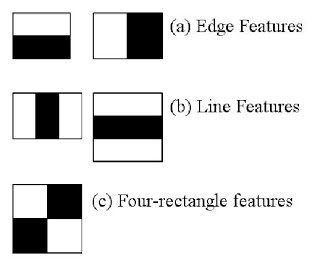
\includegraphics[width=0.5\textwidth]{images/openCv/haar_features.jpg}
\caption{Alcune haar-features.\label{features}}
\end{figure}

Le immagini vengono scansionate alla ricerca dei vari pattern di base. Ad ogni passaggio la ricerca viene ripetuta aumentando le dimensioni dei pattern. Il numero totale di feature calcolabili è molto grande, basti pensare che in un'immagine $24\times 24$ è possibile trovare più di $160.000$ feature. Per questo si procede a prendere in considerazione solamente le feature più rilevanti.
Per esempio nella figura \ref{volti} notiamo che nel volto sono stati riconosciute due particolari feature: una all'altezza degli occhi e una che ricalca la forma del naso.

\begin{figure}%[htbp]
\centering
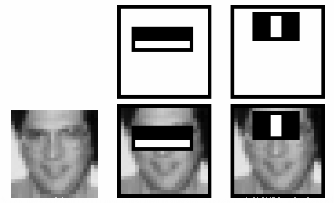
\includegraphics[width=0.5\textwidth]{images/openCv/haar.png}
\caption{Particolari features riconosciute nel volto.\label{volti}}
\end{figure}

Infatti la zona degli occhi solitamente è più scura rispetto alle altre parti del volto, ricalcando il primo pattern visibile nella figura \ref{features}, mentre il naso, posizionato tra le due zone scure degli occhi, presenta un pattern che ricalca la prima feature della seconda riga.\\
Dato un insieme di immagini positive, l'algoritmo procede a fare una classificazione per suddividere le feature simili in classi uguali, con una soglia prestabilita. Si selezionano solamente le feature con rapporto di errore minimo, in modo da suddividere quelle che possono ricondurre alle caratteristiche di un volto da quelle che non fanno parte di esso.\\
Le immagini vengono scansionate fino a che il tasso di errore rimane sotto una certa soglia oppure in base al numero di stages di classificazione deciso dall'utente. Alla fine del processo tutti i risultati, ovvero le features, vengono salvati all'interno di un file XML, che rappresenta il cascade desiderato.\\
OpenCv offre dei metodi, come \texttt{detect\_multiscale()}, che permettono di riconoscere oggetti, scansionando un'immagine con lo scopo di cercare le features descritte nel cascade. 


\end{itemize}




\section{OpenGl}

\begin{figure}[hbp]
\centering

\includegraphics[width=0.7\textwidth]{images/openGL/OpenGL_logo.jpg}
\end{figure}


OpenGL (Open Graphics Library) è una specifica che definisce un'API (“Application Programming Interface”, “interfaccia di programmazione per applicazioni”) che fornisce metodi per sviluppare applicazioni di grafica 2D e 3D \cite{opengl-wiki}. E' stata introdotta nel 1992 dalla società californiana Silicon Graphics, è nata in ambiente Unix e, successivamente, è stata resa multipiattaforma. La libreria OpenGL è usata per vari tipi di applicazioni, come animazioni, videogiochi, simulazioni 3D e di realtà virtuale.

Una specifica è un documento che descrive un insieme di funzioni ed il comportamento preciso che queste devono avere. I maggiori produttori hardware (Nvidia, AMD, Intel, etc) creano implementazioni di queste funzioni rispettando la specifica OpenGL, usando l'accelerazione hardware quando possibile. In questo modo il programmatore può usufruire di un'API unificata, utilizzando le funzioni senza preoccuparsi della loro implementazione.

Un'altra caratteristica fondamentale è che le funzioni di OpenGL devono essere sempre usufruibili, quindi le implementazioni richiedono un'emulazione software quando l'hardware non è in grado di fornire certe funzionalità.

\subsection{Il funzionamento di OpenGL}
OpenGL offre circa 250 chiamate di funzione per disegnare scene a due  o tre dimensioni, a partire da delle primitive. Con primitive si intendono punti, linee e poligoni, i quali vengono convertiti in pixel tramite una serie di processi chiamata pipeline grafica.
La pipeline rappresenta una catena di trasformazioni e operazioni, in cui ogni fase prende in input il risultato della fase precedente e produce l'output per la fase successiva.

OpenGL opera a basso livello e richiede al programmatore di rispettare i passi precisi della pipeline che servono a renderizzare la scena. Tra i passi principali da seguire sono presenti :

\begin{itemize}
\item fornire le primitive che descrivano la scena.
\item fornire le regole per generare una telecamera virtuale, che renderizzi solo determinate porzione della scena, con particolari modalità.
\item fornire le regole per gestire texture, materiali, luci e ombre.
\end{itemize}

Queste regole vanno definite in particolari file chiamati "shader", scritti in un linguaggio ad alto livello proprio di OpenGL, basato sul linguaggio C, chiamato GLSL ("OpenGL Shading Language"). Siccome la scena non può essere renderizzata senza aver fornito le regole basilari, è necessaria, da parte del programmatore, una buona conoscenza della suddetta pipeline grafica e del linguaggio GLSL.

Esistono anche framework che operano ad alto livello, i quali nascondono al programmatore le fasi più complesse del rendering, gestendole autonomamente, e richiedono solamente una descrizione generica della scena. Un'esempio è il framework Ogre3D, trattato in seguito.

\clearpage



\section{Ogre3D}
\textbf{Ogre3D} (“Object-Oriented Graphics Rendering Engine”) è un motore grafico 3D open-source, scritto in C++, che essenzialmente offre un'API che sfrutta l'accelerazione hardware per la creazione di applicazioni grafiche. 

\begin{figure}
\centering

\includegraphics[width=0.6\textwidth]{images/ogre/ogrelogo-small.jpg}

\end{figure}

\subsection{Storia}
E' stato ideato nel 1999 da uno sviluppatore inglese di nome \textbf{Steve Streeting}, dopo che ebbe creato un progetto chiamato \textbf{DIMClass}, il quale aveva lo scopo di rendere più semplice l'utilizzo della libreria Direct3D. Si rese conto che il livello di astrazione raggiunto dalla sua libreria era cosi elevato che non aveva più bisogno di essere basata su Direct3D. Da qui nacque l'idea di creare una libreria che fosse indipendente da API a basso livello \cite{ogre-wiki}.

Nel 2000 il progetto fu registrato su \textbf{SourceForge}\footnote{ Piattaforma web per lo sviluppo di progetti e software, facilitando la collaborazione tra sviluppatori }, con il nome di OGRE. Il 25 febbraio 2005 fu rilasciata la  prima versione di Ogre, la 1.0.0, con il nome di “Azathoth”. La versione utilizzata in questo progetto è la 1.9.0, rilasciata il 24 novembre 2013, con il nome “Ghadamon”.

\subsection{La struttura ad albero}
Ogre3D utilizza una struttura dati ad albero (\textbf{scene graph}), dove ogni nodo può avere più figli ma un solo padre. Ogni nodo permette di gestire determinate caratteristiche della scena, e ogni suo comportamento si riflette in tutti i suoi discendenti. I principali nodi sono, a partire dalla radice e procedendo gerarchicamente:
\begin{itemize}
\item \textbf{Root}: permette di configurare il sistema.
\item \textbf{Scene Manager}: gestisce tutta la scena. Solitamente si usa un solo Scene Manager, ma è possibile crearne altri. Utilizzare più Scene Manager permette di renderizzare la scena in modo diverso; questo può essere usato ad esempio per suddividere la finestra in più parti, ognuna delle quali inquadra una zona diversa della scena (split screen).
\item \textbf{Scene Node}: appendendo diversi oggetti a questo nodo, è possibile creare gruppi di elementi, in modo da poter applicare effetti o trasformazioni all'intero gruppo, utilizzando una singola istruzione.
\item \textbf{Oggetti}: tra i singoli oggetti utilizzabili, i principali sono le telecamere (\textbf{Camera}), le luci (\textbf{Light}) e le entità (\textbf{Entity}). Queste ultime rappresentano i modelli 3D, che possono essere importati dall'esterno, o creati grazie a metodi che costruiscono primitive quali piani o cubi. 
\end{itemize}
%Ogre3D utilizza una struttura dati ad albero (\textbf{scene graph}), dove ogni nodo può avere più figli ma un solo padre. Partendo dalla radice, che permette di configurare il sistema, si possono poi creare dei figli che gestiscono la scena diversamente. Il nodo principale è lo \textbf{Scene Manager} che, come dice il nome, gestisce tutto ciò che è presente nella scena. Solitamente si utilizza un solo Scene Manager, ma è sempre possibile crearne di altri, magari in applicazioni più complesse, per gestire più scene. Questo può essere utilizzato ad esempio per suddividere la finestra in più parti, ognuna delle quali riprende una zona diversa della scena (split screen).
%
%Dallo Scene Manager è possibile appendere dei nodi chiamati \textbf{Scene Node}, ai quali, a loro volta, possono essere collegati elementi come entità (i modelli), luci, telecamere, etc. In questo modo è possibile raggruppare più elementi ed applicare all'intero gruppo effetti o trasformazioni con una singola istruzione.
%
%Infine troviamo i singoli oggetti. Tra questi vi sono i modelli, rappresentati da oggetti chiamati \textbf{Entity}, i quali devono essere imparentati ad almeno uno Scene Node, tramite il quale sono gestiti. E' possibile creare dei modelli preimpostati, come ad esempio cubi o piani, oppure si possono importare dall'esterno. Tra gli altri oggetti utilizzabili, i più comuni sono luci e telecamere.

\subsection{I vantaggi del framework}
Ogre3D è un framework che permette di astrarre tutta la parte che deve essere implementata in API a basso livello. Infatti, molte operazioni che devono essere esplicitate negli altri casi, qui sono gestite automaticamente: utilizzando solamente poche righe di codice è possibile richiamare metodi che implementano queste operazioni, nascondendole all'utente.
Un esempio è la creazione di modelli: Ogre3D offre dei metodi che costruiscono figure di base, oppure permettono di importare modelli sotto forma di file con estensione “.mesh”. Tutta la parte relativa al processamento dei vertici e al loro salvataggio nei buffer, viene nascosta.

Per quanto riguarda texture, materiali, luci ed ombre, Ogre3D contiene di default degli algoritmi di shading che li gestiscono. Anche la telecamera virtuale è gestita dal framework: all'utente viene richiesta solamente l'impostazione dei valori che la definiscono, mentre tutta la parte relativa alle trasformazioni viene nascosta.

Se da una parte l'autonomia del sistema porta a dei vantaggi, questo può determinare anche delle limitazioni. Fortunatamente Ogre3D lascia comunque ampie libertà: ad esempio l'utente può utilizzare materiali\footnote{I materiali sono descritti in file con estensione .material, tramite un linguaggio proprio di Ogre3D, di facile comprensione.} e shader personalizzati o preimpostati, forniti da Ogre3D al momento dell'installazione. Un altro esempio è la possibilità di definire la telecamera virtuale tramite matrici personalizzate. In particolare è possibile impostare la view matrix e la projection matrix, aspetto fondamentale ai fini della nostra applicazione. 
%
% All'utente viene comunque lasciata un'ampia libertà in quanto può utilizzare anche shader preimpostati, forniti da Ogre3D, oppure shader personalizzati, da includere nelle risorse del programma che si vuole creare.
%
%
%
%Inoltre in OpenGL la gestione di texture, ombre e materiali va implementata a mano scrivendo gli algoritmi di "shading", che contengono informazioni quali il colore o regole di comportamento in presenza di luce. Al contrario in Ogre la gestione di questi aspetti è quasi automatica in quanto di default vengono utilizzati shader già presenti nel framework.
%
%Tuttavia, Ogre è anche versatile perchè lascia all'utente ampie libertà, permettendogli di personalizzare diversi aspetti. Ad esempio in Ogre la view matrix e la perspective matrix, che servono a definire la telecamera, sono generate in automatico, in modo trasparente al programmatore. Poichè la nostra trasformazione richiedeva che le due matrici fossero in funzione della posizione dell'utente, esse sono state calcolate in una funzioni scritte a mano, e poi passate come parametro a due metodi che impostano le trasformazioni a partire da matrici personalizzate.
%
%Inoltre è sempre possibile utilizzare shader personalizzati, e definire i materiali degli oggetti in file con estensione .material, scritti con un linguaggio di facile comprensione, proprio di Ogre.
%
%Per questo, una volta compresa la trasformazione che richiedeva il nostro progetto, è stata abbandonata l'idea di utilizzare OpenGL passando invece a Ogre3D, con lo scopo di concentrarci sulla qualità e la miglior resa della scena.




\chapter{frustum}
\fancyhead[RO]{\bfseries frustum}

Come abbiamo già detto, le applicazioni grafiche eseguono una serie di operazioni e trasformazioni, chiamata pipeline grafica per renderizzare una scena prelevata da un mondo virtuale 3D così come noi la vediamo a schermo. Nella figura \ref{pipeline} sono presenti le principali fasi della pipeline.

\begin{figure}[htbp]
\centering
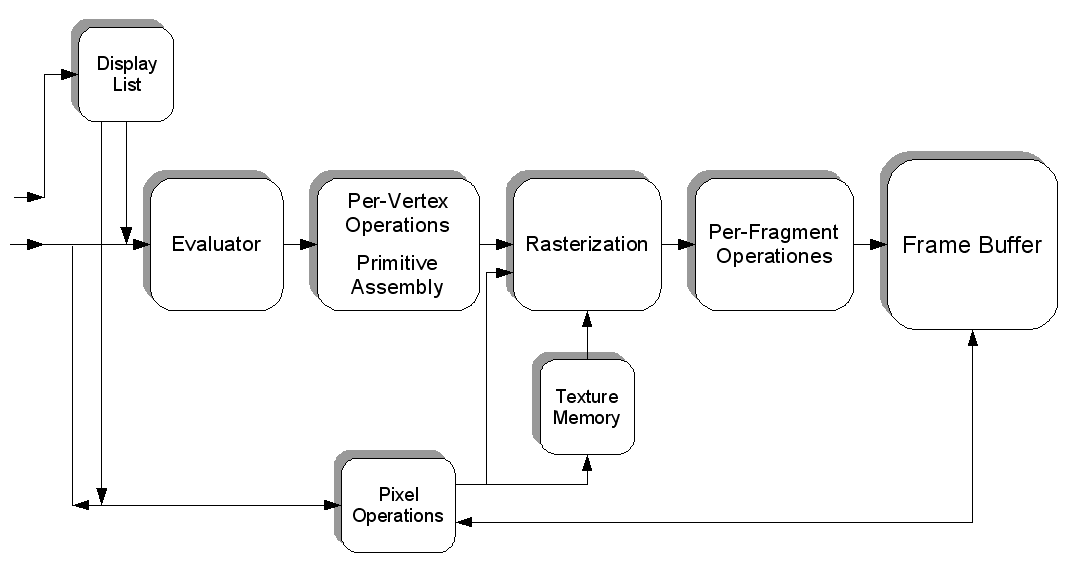
\includegraphics[width=0.7\textwidth]{images/frustum/opengl-pipeline.png}
\caption{La pipeline grafica.\label{pipeline}}
\end{figure}

Ai fini di questo progetto, ci concentreremo sulle trasformazioni, più che su altre operazioni come la rasterizzazione (conversione da vettori a pixel, costruendo segmenti o porzioni di piano che riempiono lo spazio definito da due o più vertici) o l'applicazione di materiali e texture.

\section{Le trasformazioni}
Il diagramma in figura \ref{trans-pipe} mostra le principali trasformazioni eseguite nella pipeline.

\begin{figure}[htbp]
\centering
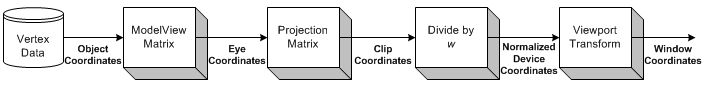
\includegraphics[width=0.7\textwidth]{images/frustum/transform-pipeline.png}
\caption{Le trasformazioni.\label{trans-pipe}}
\end{figure}

Per determinare la posizione di ciascun vertice all'interno del mondo virtuale, viene adottato un sistema di coordinate a 3 dimensioni (figura \ref{cartesian}).
\begin{figure}[htbp]
\centering
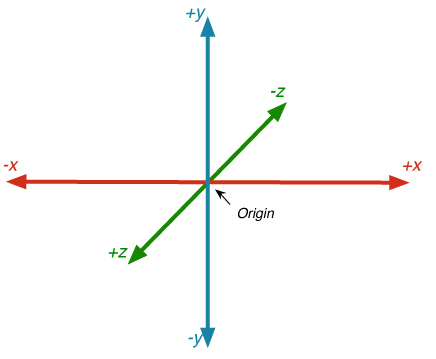
\includegraphics[width=0.3\textwidth]{images/frustum/cartesian.png}
\caption{Il sistema cartesiano in OpenGL e Ogre3D.\label{cartesian}}
\end{figure}

Da notare l'asse Z, la cui direzione positiva è quella uscente, ovvero quella rivolta verso l'utente che sta di fronte allo schermo. Questa caratteristica è fondamentale perchè determina il segno di alcuni elementi nel processo di trasformazione.

\subsection{ModelView Matrix}
Nel prima fase si utilizza una matrice chiamata Modelview Matrix, che trasforma le coordinate locali degli oggetti presenti nella scena nel sistema globale di coordinate relativo al mondo virtuale. Di default, la telecamera virtuale che inquadra la scena è posizionata nell'origine del sistema, ovvero nel punto $(0,0,0)$. La telecamera punta lo sguardo verso l'asse -Z, mentre gli assi X e Y sono paralleli al piano che rappresenta lo schermo (figura \ref{cam-default}).

\begin{figure}[htbp]
\centering
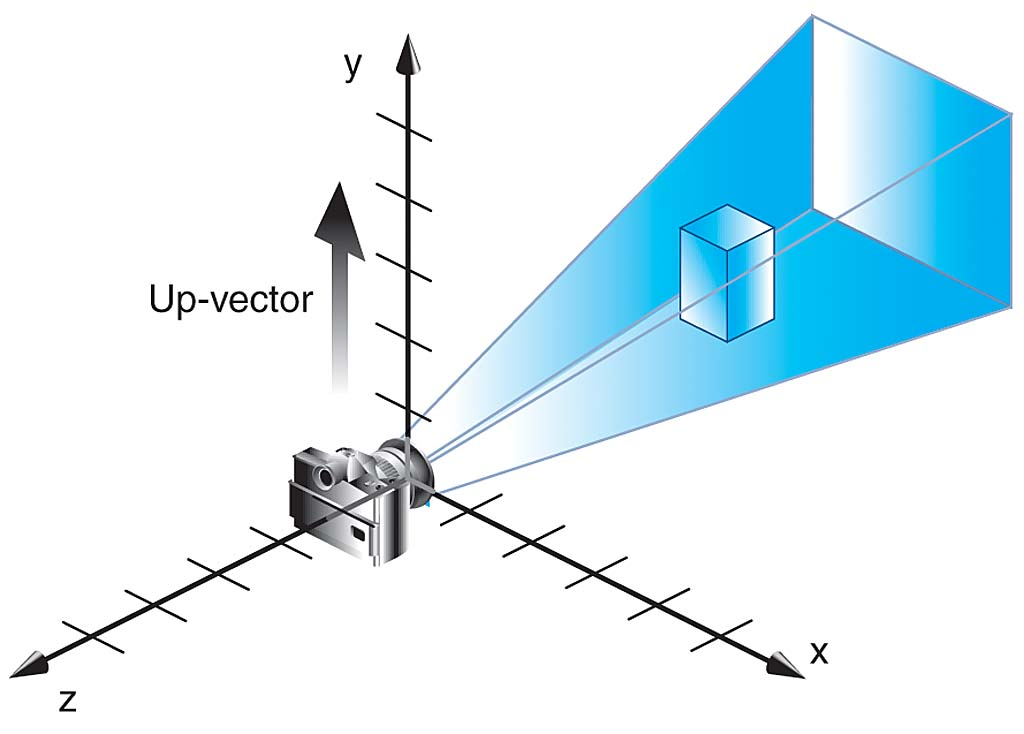
\includegraphics[width=0.5\textwidth]{images/frustum/camera-default.jpg}
\caption{La posizione di default della telecamera virtuale.\label{cam-default}}
\end{figure}


\subsection{Projection Matrix}
Lo spazio che identifica la porzione del mondo che è possibile osservare, è chiamato view volume (figura \ref{view-frustum}); tutto ciò che si trova all'interno di esso viene renderizzato nella scena.

\begin{figure}[htbp]
\centering
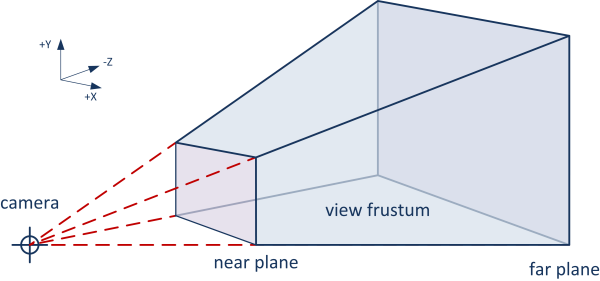
\includegraphics[width=0.5\textwidth]{images/frustum/view_frustum.png}
\caption{Il view volume nella proiezione prospettica.\label{view-frustum}}
\end{figure}

Questo spazio è caratterizzato da un piano più vicino alla telecamera, il near plane, e uno più lontano, il far plane. Il near plane rappresenta la coordinata Z dalla quale sarà renderizzata la scena, ovvero tutto ciò che sta dietro non sarà visibile. Il far plane rappresenta la coordinata Z di fine scena, perciò determina quanto in profondità essa è visibile.

La Projection Matrix ha il compito di trasformare il view volume in un cubo $2 \times 2\times 2$ centrato nell'origine, determinando anche la trasformazione di tutto ciò che è presente al suo interno. Ogni vertice all'interno di esso avrà coordinate $-1\leq x,y,z \leq 1$.

Il modo in cui viene considerato il view volume, e quindi il modo in cui viene trasformato lo spazio, dipende dal tipo di proiezione. Essenzialmente esistono due tipi di proiezione, quella ortogonale e quella prospettica.

\begin{figure}[htbp]
\centering
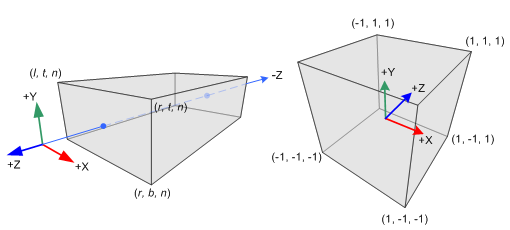
\includegraphics[width=0.5\textwidth]{images/frustum/orto-projection.png}
\caption{Trasformazione con proiezione ortogonale.\label{orto}}
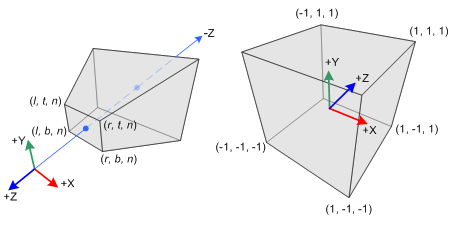
\includegraphics[width=0.5\textwidth]{images/frustum/persp-projection.png}
\caption{Trasformazione con proiezione prospettica.\label{persp}}
\end{figure}

In quella ortogonale (figura \ref{orto}) il view volume è rappresentato da un parallelepipedo; in questo caso tutti i vertici vengono proiettati sul near plane, parallelamente alla direzione della telecamera. Il risultato sarà quello di avere una visione non prospettica della scena.

La proiezione prospettica (che vedremo in dettaglio in seguito, in quanto il suo uso è fondamentale in questo progetto) presenta un view volume che ha la forma di un tronco di piramide, in inglese frustum.
Il vertice della piramide è dato dalla posizione della telecamera, mentre il near plane e il far plane sono rispettivamente la base minore e maggiore del frustum. In questo caso i vertici vengono proiettati sul near plane seguendo la direzione che li congiunge alla telecamera. Dopo aver applicato questa trasformazione, il frustum diventerà un cubo, e tutti gli oggetti al suo interno saranno deformati per come sono visti a schermo.

Nelle figure \ref{example1} e \ref{example2} è possibile vedere un esempio di questa trasformazione.
\begin{figure}[htbp]
\centering
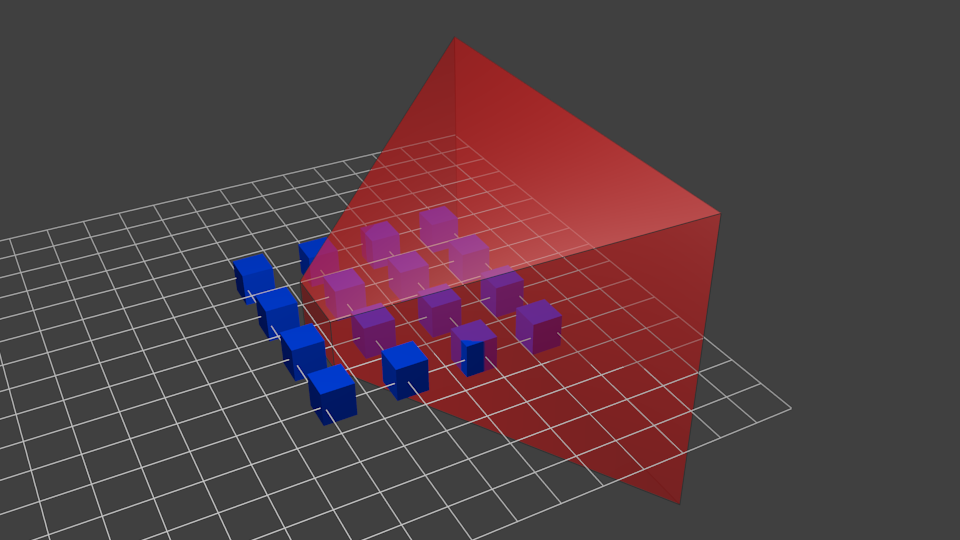
\includegraphics[width=0.6\textwidth]{images/frustum/frustum_cubes.png}
\caption{Il frustum prima della trasformazione.\label{example1}}
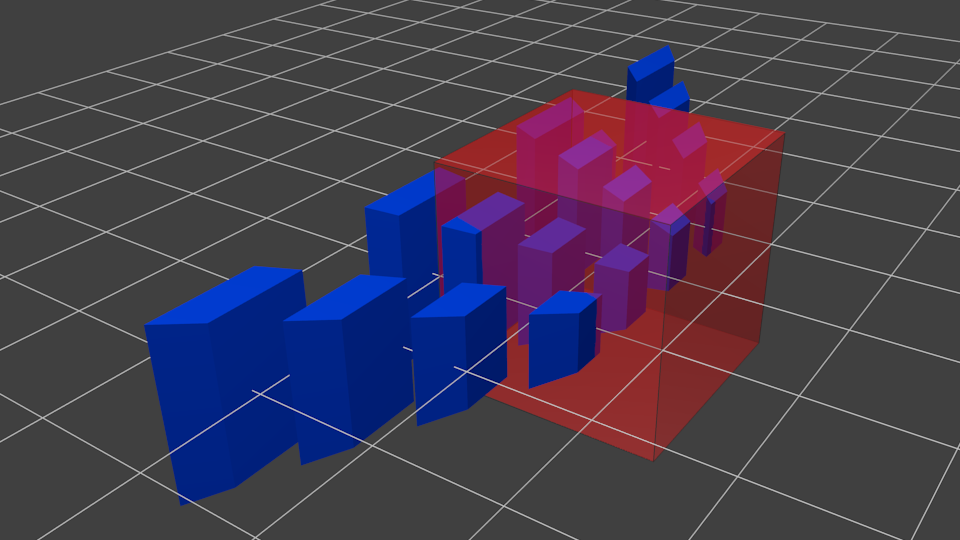
\includegraphics[width=0.6\textwidth]{images/frustum/frustum_homogeneous.png}
\caption{Il frustum trasformato nel sistema di coordinate omogeneo.\label{example2}}
\end{figure}

Nella figura \ref{example3} il cubo è visto dal suo piano frontale.

\begin{figure}[htbp]
\centering
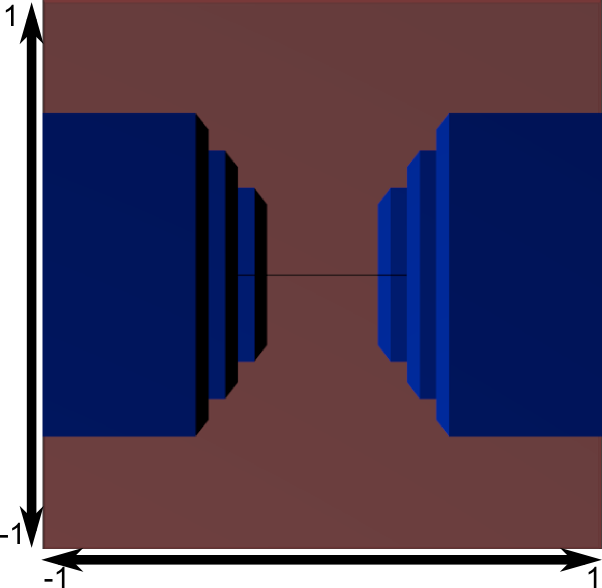
\includegraphics[width=0.5\textwidth]{images/frustum/frustum_view.png}
\caption{Il nuovo frustum visto in prospettiva.\label{example3}}
\end{figure}

Nella projection matrix è compresa l'operazione che normalizza i vertici, mappando le coordinate in modo che siano comprese tra $-1$ e $1$. Questa normalizzazione è data da una divisione delle componenti di ogni vertice per la quarta componente, cioè la coordinata W.


L'utilizzo della quarta coordinata per definire i vertici dà origine al sistema di coordinate omogenee. Questo sistema, introdotto da August Ferdinand Möbius intorno al 1837, prevede la rappresentazione di $N$ coordinate con vettori di $N+1$ dimensioni, ed è usato per descrivere i punti nella geometria proiettiva. Inoltre la quarta coordinata permette di rappresentare tutte le trasformazioni affini (trasformazioni lineari più una traslazione) tramite le matrici.

Considerando che la traslazione di un vettore a due dimensioni $v = (x,y)$ per un vettore $v_0 = (a,b)$
è data dalla loro somma, è possibile rappresentare questa trasformazione anche tramite una matrice $3\times3$:
$$T_{v_0} \times v = \begin{pmatrix} 1 & 0 & a \\
0 & 1 & b \\
0 & 0 & 1
\end{pmatrix}
\begin{pmatrix}
x \\
y \\
1 
\end{pmatrix}
=
\begin{pmatrix}
x + a \\
y + b \\
1
\end{pmatrix}$$\\

E' possibile estendere questo concetto ad ogni tipo di trasformazione, permettendo di raggruppare più trasformazioni in una singola matrice uguale al prodotto delle matrici che le rappresentano.

\subsection{Viewport Matrix}
L'ultimo passaggio è dato dalla Viewport Matrix, che trasforma i vertici in coordinate relative allo schermo. Dopo questa fase, il nuovo sistema di riferimento è relativo all'angolo in basso a sinistra della finestra aperta dopo aver lanciato l'applicazione, e le coordinate sono date dai pixel dello schermo.

Dati i valori \textit{w} (width = larghezza) e \textit{h} (height = altezza), in pixel, il canonical view volume viene ridotto, scalandolo di $w/2$ nella direzione orizzontale e di $h/2$ nella direzione verticale. Dopo di ciò il tutto viene traslato di un vettore $(-w/2, -h/2, -1)$ per allineare l'angolo in basso a sinistra di fronte del canonical view volume (cioè il punto $(-1,-1,-1)$) con l'angolo in basso a sinistra della finestra visualizzata a schermo.

Tutte le operazione che si svolgono dopo, come la rasterizzazione e lo shading, vengono fatte usando questo sistema di riferimento.

\section{La teoria matematica delle trasformazioni}

\subsection{Il view frustum}
Con view frustum indichiamo il view volume utilizzato nella proiezione prospettica, in quanto il frustum rappresenta il tronco di piramide che racchiude lo spazio visibile del mondo 3D; in genere viene chiamato allo stesso modo anche il view volume considerato nella proiezione ortogonale, ma in questo caso occorre notare che si tratta di un parallelepipedo e non un tronco di piramide.

Il view frustum è posizionato in modo che il vertice della piramide, rappresentante l'osservatore o la telecamera, giaccia sull'origine. Esso è composto da sei piani, due di questi li abbiamo già visti, e sono il near e il far plane. Gli altri quattro rappresentano le coordinate che definiscono i bordi del near plane, e sono chiamati left, right, bottom e top planes.


\begin{figure}[htbp]
\centering
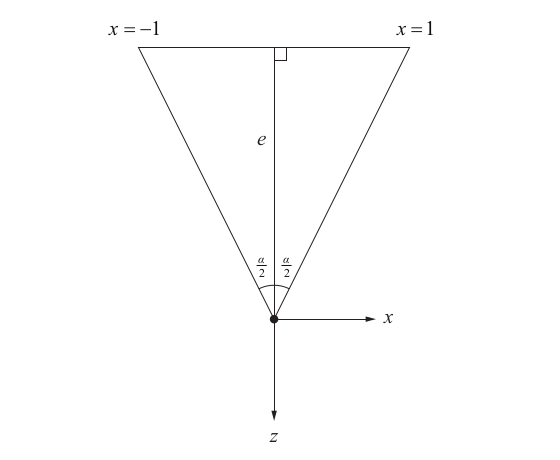
\includegraphics[width=0.6\textwidth]{images/frustum/frustum-x.png}
\caption{La distanza focale $e$ dipende dall'angolo dell'apertura $\alpha$ della telecamera. \label{frustum-x}}
\end{figure}

Si considera, in generale, che il piano di proiezione sia situato ad una distanza $e$ dall'osservatore, in modo che le coordinate del left e right plane siano rispettivamente $x=-1$ e $x=+1$ (figura \ref{frustum-x}).

La distanza $e$ è la distanza focale, che è determinata dall'angolo di apertura $\alpha$ della telecamera: valori più alti di $\alpha$ determinano valori di $e$ più piccoli, e ciò si traduce in un accorciamento della distanza e allargamento della visuale, creando un effetto grandangolare, in quanto il piano di proiezione è piu vicino all'osservatore; viceversa valori alti di $e$ determinano un allontanamento del piano di proiezione, con effetto di allungamento della distanza e restringimento della visuale.

Grazie alla trigonometria possiamo calcolare la distanza focale a partire dall'angolo di apertura, come  $$e = \frac{1}{\tan(\alpha/2)}$$.

Un altro valore da tenere in considerazione è l'aspect ratio , cioè il rapporto tra la lunghezza e l'altezza del piano. Per esempio in uno schermo $1920\times 1080$ l'aspect ratio è uguale $\frac{1080}{1920}=\frac{16}{9}$, oppure in uno schermo $640\times 480$ è $\frac{640}{480}=\frac{4}{3}$.Grazie a questo possiamo determinare il formato della finestra che vogliamo visualizzare a schermo.

\begin{figure}[htbp]
\centering
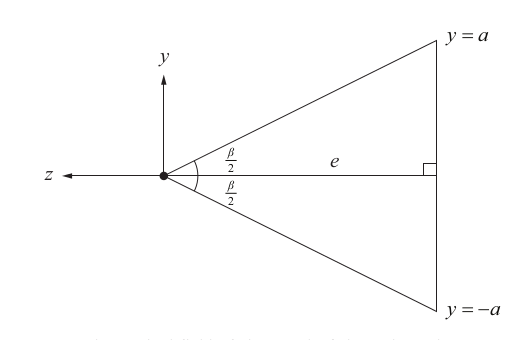
\includegraphics[width=0.6\textwidth]{images/frustum/frustum-y.png}
\caption{L'angolo di apertura verticale $\beta$ dipende dall'aspect ratio.\label{frustum-y}}
\end{figure}

Considerando che il left e right plane hanno coordinate $x=-1$ e $x=+1$, il bottom e top plane vengono posizionati alle coordinate $y=-a$ e $y=+a$, dove $a$ è il reciproco dell'aspect ratio; nel caso $\frac{16}{9} \rightarrow a=\frac{9}{16}=0.5625$ (figura \ref{frustum-y}).

Possiamo calcolare l'angolo di apertura verticale $\beta$ come: $$\beta=2\tan^{-1}(a/e)$$ 

Possiamo assegnare arbitrariamente un valore $n$ come coordinata per il near plane, in modo da determinare la distanza da cui inizia il frustum. Le coordinate dei quattro piani ora devono essere ricalcolate come $$x =\pm \frac{n}{e}$$ e $$y = \pm \frac{an}{e}$$.



\subsection{Projection Matrix}
Come abbiamo detto all'inizio del capitolo, per renderizzare a schermo un punto tridimensionale, esso deve essere trasformato in un punto a due dimensioni. Il sistema di coordinate omogenee,  che si utilizza per identificare i punti nello spazio, possiede quattro dimensioni. La projection matrix lo trasforma in un sistema a tre dimensioni, proiettando lo spazio omogeneo in uno spazio 3D chiamato canonical view volume (un cubo).

Dopo aver proiettato i punti omogenei sul near plane, le nuove coordinate vengono normalizzate, cioè divise per la quarta coordinata $w$; questo permette di mappare le nuove coordinate in uno spazio $[-1,1]$.

Consideriamo un punto omogeneo $P=\langle P_x,P_y,P_z,1\rangle$ situato nel view frustum.
Riprendendo il discorso del paragrafo precedente riguardante i triangoli simili,  le coordinate $x$ e $y$ del punto proiettato sul near plane sono
\begin{center}
$x=-\frac{n}{P_z}{P_x}$ \,\,\,e\,\,\,  $y=-\frac{n}{P_z}{P_y}$
\end{center}
$$\begin{array}{cc}
x=-\frac{n}{P_z}{P_x} & y=-\frac{n}{P_z}{P_y}\\
\end{array}$$\\


Allora $l\leq x\leq r$ e $b\leq y\leq t$, dove l,r,b,t sono le coordinate dei quattro piani del frustum, descritti in precedenza.
Per mappare le nuove coordinate x e y si usano le funzioni lineari:
$$x'=(x-l)\frac{2}{r-l}-1$$ e $$y'=(y-b)\frac{2}{t-b}-1$$
Sostituendo alla x e alla y le espressioni scritte in precedenza e semplificando otteniamo:
$$x'=\frac{2n}{r-l}\left(-\frac{P_x}{P_z}\right)-\frac{r+l}{r-l}$$ e 
$$y'=\frac{2n}{t-b}\left(-\frac{P_y}{P_z}\right)-\frac{t+b}{t-b}$$\\
Per quanto riguarda la mappatura della coordinata z, si deve trovare una funzione che porti $-n\rightarrow -1$ e $-f\rightarrow 1$.
Considerando che le coordinate z hanno i reciproci interpolati, possiamo scrivere una funzione di $1/z$:
$$z'=\frac{A}{z}+B$$
Abbiamo detto che $-n\rightarrow -1$ e $-f\rightarrow 1$, perciò possiamo ottenere il sistema:
$$-1=\frac{A}{-n}+B$$ e $$1=\frac{A}{-f}+B$$
Risolvendo il sistema otteniamo:
$$A=\frac{2nf}{f-n}$$ e $$B=\frac{f+n}{f-n}$$\\
Sostituendo $A$ e $B$:
$$z'=-\frac{2nf}{f-n}\left(-\frac{1}{P_z}\right)+\frac{f+n}{f-n}$$
Si può notare che nelle equazioni di $x'$, $y'$ e $z'$ è presente una divisione per $-P_z$: il punto tridimensionale $P'=\langle x',y',z'\rangle$ è equivalente al punto omogeneo 4D $P=\langle -x'P_z,-y'P_z,-z'P_z,-P_z\rangle$ dopo che esso viene diviso per la sua coordinata w, cioè per $-P_z$.
Perciò possiamo esprimere le precedenti equazioni mettendo in evidenza $-x'P_z$, $-y'P_z$, e $-z'P_z$:
$$-x'P_z=\frac{2n}{r-l}P_x+\frac{r+l}{r-l}P_z$$, 
$$-y'P_z=\frac{2n}{t-b}P_y+\frac{t+b}{t-b}P_z$$e
$$-z'P_z=-\frac{f+n}{f-n}P_z-\frac{2nf}{f-n}$$

Essendo funzioni lineari delle coordinate del punto $P$, possiamo utilizzare una matrice $4\times 4$ per rappresentare la trasformazione prospettiva; moltiplicando la matrice per il punto P, otteniamo la sua proiezione $P'$ sul near plane:
$$P'=M*P=
\begin{bmatrix}
\frac{2n}{r-l} & 0 & \frac{r+l}{r-l} & 0 \\
0 & \frac{2n}{t-b} & \frac{t+b}{t-b} & 0 \\
0 & 0 & -\frac{f+n}{f-n} & -\frac{2nf}{f-n} \\
0 & 0 & -1 & 0
\end{bmatrix}
\begin{bmatrix}
P_x \\ P_y \\ P_z \\ 1
\end{bmatrix}$$

In OpenGL esistono essenzialmente due funzioni per generare una matrice di proiezione prospettica: la libreria GLM (OpenGL Mathematics), usata in questo progetto (nella versione sviluppata in OpenGL), offre i metodi \texttt{perspective(float fov, float aspect, float n, float f)}
e \texttt{glFrustum(float l,float r,float t,float b,float n,float f)}.

La prima funzione restituisce una matrice di proiezione con frustum simmetrico, ovvero il near plane assume la figura di un rettangolo; questo è il tipo di frustum maggiormente utilizzato; come visto all'inizio del paragrafo relativo al view frustum, tramite l'angolo di apertura di campo fov, e l'aspect ratio, è possibile calcolare le coordinate dei quattro piani del frustum, oltre al near e il far. Dopo aver calcolato le coordinate, la funzione genera la matrice desiderata.

La seconda funzione invece prende in input le coordinate dei sei piani del frustum e calcola direttamente la matrice; in questo modo è anche possibile creare un frustum asimmetrico, generando una prospettiva distorta (il near plane può assumere la forma di un quadrilatero qualsiasi).

Quest'ultima funzione è stata utilizzata in questo progetto, in modo da avere la possibilità di distorcere la prospettiva della scena in base alla posizione dell'osservatore.  

\subsection{View Matrix}
La Projection Matrix trasforma lo spazio considerando che la telecamera sia situata nell'origine e che la direzione dello sguardo sia rivolto lungo l'asse negativo delle Z. Per questo, se la telecamera è posizionata in punti diversi, si deve applicare un'altra trasformazione, che porti la telecamera nella sua posizione di default. Questa trasformazione è data dalla View Matrix, che ha il compito di trasformare lo spazio di coordinate del mondo 3D nello spazio di coordinate relativo alla telecamera. In pratica la telecamera viene ruotata e traslata per essere posizionata nell'origine, con il corretto orientamento, e nello stesso momento tutto il mondo 3D subisce la stessa trasformazione (figure \ref{view1} e \ref{view2}).

\begin{figure}[htbp]
\centering
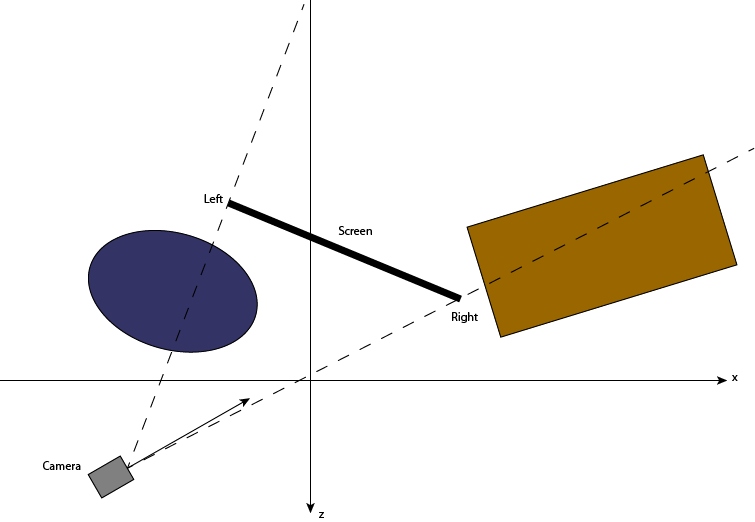
\includegraphics[width=0.5\textwidth]{images/frustum/view-matrix1.png}
\caption{Una scena con la telecamera posta in un punto qualsiasi.\label{view1}}
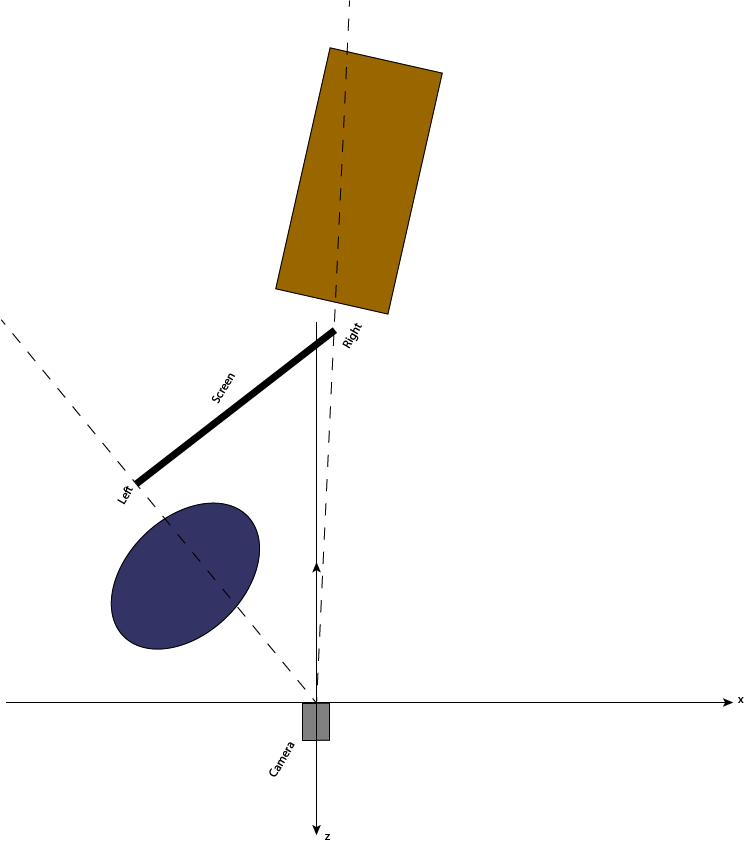
\includegraphics[width=0.5\textwidth]{images/frustum/view-matrix2.png}
\caption{La scena trasformata con la view matrix.\label{view2}}
\end{figure}


Dopo aver applicato questa trasformazione è possibile applicare anche la proiezione.

Il calcolo della view matrix necessita di tre vettori:
\begin{itemize}
\item \textbf{eye}: identifica la posizione della telecamera.
\item \textbf{target}: identifica il punto verso cui è rivolto lo sguardo.
\item \textbf{up}: identifica la direzione che punta verso l'alto, di solito coindice con l'asse y, quindi è $(0, 1, 0)$.
\end{itemize}

La matrice consiste in due trasformazioni: una rotazione, per allineare l'orientamento della telecamera con l'asse negativo delle Z, e una traslazione, per spostare la telecamera nell'origine.
Per la rotazione si calcola una base ortonormale che rappresenta il sistema di coordinate relativo alla telecamera, tramite i tre vettori, ponendo\\
$n = normalize(eye - target)$\\
$u = normalize(cross(up,n))$\\
$v = cross(n,u)$\\
dove $cross(a,b)$ rappresenta il prodotto vettoriale tra $a$ e $b$ e $normalize(a)$ la normalizzazione di $a$. I vettori u,v,n formano la base ortonormale desiderata.

La matrice che orienta la scena nel modo corretto è:
$$R=
\begin{bmatrix}
u.x && u.y && u.z && 0\\
v.x && v.y && v.z && 0\\
n.x && n.y && n.z && 0\\
0 && 0 && 0 && 1\\
\end{bmatrix}
$$

Per quanto riguarda la traslazione basta utilizzare la matrice

$$T=
\begin{bmatrix}
0 && 0 && 0 && -eye.x\\
0 && 0 && 0 && -eye.y\\
0 && 0 && 0 && -eye.z\\
0 && 0 && 0 && 1\\
\end{bmatrix}
$$\\
dove il meno permette di traslare la scena in modo che la telecamera finisca nell'origine.

La View Matrix è data dal prodotto della matrice dell'orientamento per quella di traslazione.
Possiamo perciò scriverla in modo compatto come:
$$V = R \times T =
\begin{bmatrix}
u.x && u.y && u.z && -dot( u, eye )\\
v.x && v.y && v.z && -dot( v, eye )\\
n.x && n.y && n.z && -dot( n, eye )\\
0 && 0 && 0 && 1\\
\end{bmatrix}
$$\\
dove $dot(a,b)$ rappresenta il prodotto scalare tra $a$ e $b$.





\chapter{Il progetto}
\fancyhead[RO]{\bfseries Il progetto}

L'obiettivo del progetto è quello di offrire un'interfaccia uomo-macchina, che permetta all'utente di interagire con la telecamera virtuale della scena, utilizzando il proprio volto come controller. Utilizzando la tecnica dell'head-tracking viene rilevato il volto, il  movimento del quale determina la trasformazione della prospettiva con cui è visualizzata la scena, generando l'illusione della presenza di profondità al di là dello schermo. Con un rilevamento efficiente del volto, e con una scena ben fatta, è possibile creare una visione tridimensionale senza l'uso di occhialini 3D.

L'applicazione è stata sviluppata in due versioni, utilizzando due API differenti: OpenGL e Ogre3D.

La prima versione è il risultato dello studio di fattibilità e può essere considerato un prototipo.
Utilizzare OpenGL, il quale lavora a basso livello, è stato utile per comprendere meglio il comportamento del sistema in base alle trasformazioni adottate. La scena creata rappresenta l'interno di una scatola, con la parte frontale aperta posizionata sul near plane, in modo da dare l'illusione che lo stesso schermo del PC sia l'apertura della stessa; all'interno sono stati aggiunti dei semplici cubi.

La seconda versione è stata sviluppata una volta compresi i principi delle trasformazioni adottate. L'utilizzo di Ogre3D ha portato a dei miglioramenti in termini di grafica, grazie alla possibilità di importare facilmente scene create tramite altri software di modellazione. Visto che questa versione presenta anche dei miglioramenti in termini di efficienza, la prenderemo in esame ed analizzeremo il suo codice, trattando le fasi principali in dettaglio.
In seguito sarà dedicata una sezione all'importazione delle scene in Ogre.


L'applicazione è stata scritta in C++ ed è divisa in due parti principali:
\begin{itemize}
\item Un modulo OpenCV separato da tutto il resto, che offre un metodo che fornisce le coordinate del volto rilevate nel momento in cui viene richiamato.
\item La parte grafica sviluppata usando Ogre3D.
\end{itemize}


\section{Il funzionamento dell'applicazione}
Il cuore dell'applicazione risiede nelle trasformazioni da applicare alla scena. In ogni frame sono eseguite diverse fasi, a partire dall'ottenimento delle coordinate del volto, arrivando a trasformare la prospettiva nel modo voluto. Vediamo in breve le fasi:
\begin{enumerate}
\item Ottenimento delle coordinate del volto, in pixel (relative alla webcam).
\item Applicazione di un filtro per eliminare il rumore generato a causa dell'imprecisione del rilevamento.
\item Trasformazione delle coordinate in punti dello spazio 3D.
\item Calcolo dei sei piani del frustum in base alle coordinate dell'osservatore, e creazione della projection matrix.
\item Calcolo dei vettori necessari per la view matrix, e creazione della stessa.
\item Creazione di una matrice di traslazione per aggiustare lo spostamento della telecamera, in modo che l'apertura della scena sia fissata ai bordi dello schermo.
\item La matrice relativa alla trasformazione finale della telecamera è data dal prodotto delle tre matrici calcolate nei tre passi precedenti.
\end{enumerate}
Analizzando in dettaglio le varie fasi:

\subsection*{Step 1: Ottenimento delle coordinate}

Grazie al modulo OpenCV, richiamando una semplice funzione possiamo ottenere le coordinate del volto in un dato frame.\\

Di seguito un estratto di codice della funzione nel modulo OpenCV.

\begin{lstlisting}
bool getFaceCoord(int* x, int* y, int* z ) {
...

  if ( detectAndDisplay( pt, z ) ) {
        *x = pt.x;
        *y = pt.y;
        *z = z;
        return true;
    } 
    return false;
}
...

bool detectAndDisplay( cv::Point& center, int& z ) {
...
face_cascade->detectMultiScale( frame_gray, faces, 1.1, 3,
                                0|cv::CASCADE_SCALE_IMAGE, 
                                cv::Size(90,110) );
    
    // se viene rilevato un solo volto
    if (faces.size() == 1 ) { 
            center.x = faces[0].x + faces[0].width*0.5;
            center.y = faces[0].y + faces[0].height*0.1;
            z = faces[0].width;
    }
    return true;
}
\end{lstlisting}
\texttt{detectMultiscale} è un metodo della classe \textit{CascadeClassifier}; il cascade utilizzato è \texttt{haarcascade\_frontalface\_default.xml}, fornito da OpenCV, il quale contiene le informazioni per rilevare volti umani. Il metodo perciò rileva i volti e inserisce i risultati in un vettore di matrici, \textit{faces}. Va controllata la dimensione del vettore \textit{faces}, in quanto il volto rilevato deve essere uno solo, per evitare di generare confusione tra le coordinate.

Successivamente si memorizzano le tre coordinate del volto:
\begin{itemize}

\item Per la $x$ si considera la coordinata $x$ del centro del volto rilevato.
\item Per la $y$ si considera la coordinata $y$ a $1/10$ dell'altezza del volto, partendo dall'alto. Con varie prove si è notato che gli occhi sono rilevati all'incirca a questa altezza.
\item Per la $z$ si considera la larghezza del volto in pixel. Purtroppo non è stato trovato un modo migliore per stimare la distanza dallo schermo, perciò ci si è accontentati di questa misurazione abbastanza grossolana.  
\end{itemize}


In seguito il codice presente nella parte Ogre3D, in cui viene richiamata la funzione descritta in precedenza:
\begin{lstlisting}
Ogre::Real x,y,z;
int coordX = 0 ,coordY = 0,coordZ = 0;
if (!getFaceCoord( &coordX, &coordY, &coordZ ) ) {
    x = flX->interpolate(prevX);
    y = flY->interpolate(prevY);
    z = flZ->interpolate(prevZ);
}
\end{lstlisting}
Il metodo \texttt{getFaceCoord()} viene richiamato passando come parametri tre interi. Se la funzione ritorna true si continua con le fasi successive, altrimenti significa che c'è stato un errore nel frame corrente e perciò vengono prese in considerazione le coordinate del frame precedente, per evitare crash o blocchi nell'applicazione.

\subsection*{Step 2: Filtro antirumore}
Come abbiamo detto nel paragrafo relativo ad OpenCV, vari fattori creano difficoltà nel tracking; fra le varie conseguenze, una è la generazione di una sorta di rumore: rimanendo fermi, le coordinate rilevate oscillano sempre di minimo 2 o 3 pixel, e questo determina un fastidioso tremolio nella scena.

Per ovviare (almeno in parte) a questi problemi, è stato creato un piccolo algoritmo che filtra il rumore generato dal rilevamento, cercando di preservare la fluidità nei movimenti. Di seguito la funzione che elimina il rumore di fondo.
\begin{lstlisting}
void Filter::filter(Ogre::Vector2 &cVec, int erMin) {
    int coord = cVec.x; //coordinata attuale
    int p     = cVec.y; //coordinata precedente
	
    // se coord = 0 il rilevamento non e' avvenuto
    // percio' si considera la coordinata precedente
    if (coord == 0) {
        cVec.x = p;
        return;
    }
    
    int dif = abs( coord - p );
    
    // se e' sotto la soglia minima salva 
    // la coordinata precedente
    if ( dif <= erMin ) {
        cVec.x = p;     	
    }
    // altrimenti pone la precedente uguale all'attuale
    else {
        cVec.y = coord;	
    }  
}
\end{lstlisting} 

La funzione prende in input un vettore con la coordinata attuale e precedente, e una soglia minima di errore.
Se la differenza in valore assoluto tra le due coordinate è minore della soglia minima, allora si scarta la nuova coordinata e si utilizza la precedente, perciò non viene generato movimento. Questo elimina il rumore, ma crea un altro problema: quando l'utente si sposta normalmente la prospettiva viene trasformata eseguendo movimenti a scatti, dovuti proprio al filtro che elimina comunque dati utili.

Per risolvere questo secondo problema è stato creato un secondo algoritmo che interpola i movimenti, rendendoli più fluidi grazie alla generazione di coordinate intermedie tra l'attuale e la precedente. Analizziamo il codice.
\begin{lstlisting}
Ogre::Real FluidFilter::interpolate(Ogre::Real c) {
    // se la coordinata rilevata e' la stessa
    // si avvicina ad essa
    if ( lastCoord == c ) {

        if (count == 1) {
            count--;
            last = c;
        }
        else if ( count > 0) {
            count--;
            last += gap;
        }
    }
    
    // altrimenti ricalcola il gap
    else {
        lastCoord = c;
        count = n;
        gap   =  ( c - last ) / n ;
        last += gap;
    }
    
    return last;
}
\end{lstlisting} 
La classe \textit{FluidFilter} contiene, fra gli attributi, un contatore e la coordinata interpolata nel frame precedente. Il contatore diminuisce quando le coordinate non cambiano, in modo da rendere l'interpolazione finita. Se le coordinate cambiano, si calcola un gap dato dalla differenza tra quella attuale e quella interpolata precedentemente, diviso per n; n influisce sulla qualità dell'interpolazione: all'aumento di n i movimenti sono più fluidi, ma, come effetto contrario, sono più rallentati. Con un valore di n pari a 3 o 4 l'effetto finale è accettabile, rendendo il delay quasi impercettibile e preservando una buona fluidità.

\subsection*{Step 3: Trasformazione delle coordinate}
Il sistema di coordinate di OpenCV è differente da quello relativo alla scena. Innanzitutto le coordinate fornite da OpenCV sono di tipo intero e dipendono dalla risoluzione della webcam: per esempio, con una risoluzione $640\times 480$, la $x$ può oscillare tra $0$ e $640$ e la $y$ tra $0$ e $480$; inoltre l'origine è situato nell'angolo in alto a sinistra della finestra. Il sistema del mondo 3D utilizza coordinate di tipo Real e l'origine si trova nel punto $(0,0,0)$. Per rendere compatibili i due sistemi deve essere applicata una conversione.

Con qualche prova di calibrazione si è infine deciso di utilizzare i seguenti calcoli per convertire le coordinate (già filtrate):
\begin{lstlisting}
    z = z / 150.0f;
    x = -( ( ( x - xCam/2 ) / 15.0f ) / (xr*ar) );
    y = -( ( ( y - yCam/2 ) / 15.0f ) / (yr*ar) );  
\end{lstlisting}  

\textit{xCam} e \textit{yCam} rappresentano le dimensioni della webcam in pixel. La prima sottrazione nella $x$ e nella $y$ trasla l'origine relativo ad OpenCV nell'orgine relativo al mondo virtuale.\\
\textit{ar} è il reciproco dell'aspect ratio della finestra aperta.\\
\textit{xr} e \textit{yr} sono rispettivamente il rapporto delle dimensioni della finestra per quelle della webcam, sempre in pixel. La divisione finale dovrebbe permettere di mantenere una proporzionalità dei movimenti utilizzando risoluzioni diverse. Per una maggiore efficienza, le coordinate dovrebbero essere calcolate anche in funzione della distanza dalla telecamera; purtroppo però questo studio è risultato troppo complesso, quindi è stato tralasciato.

\subsection*{Step 4: Projection matrix}
Una volta calcolate le coordinate effettive, queste vengono memorizzate nel vettore \textit{face}.
Tramite il vettore \textit{face}, si ricalcolano i piani del frustum nel seguente modo:
\begin{lstlisting}
    n = -face.z + nP;     //near plane
    f = n + sceneLength;  //far plane
    r = width - face.x;   //right plane
    l = r - 2*width;      //left plane
    t = height - face.y;  //top plane
    b = t - 2*height;     //bottom plane

\end{lstlisting}

Il near plane è calcolato in base alla distanza (approssimata) dell'osservatore, in modo che, quando questo si avvicina allo schermo, si crea un effetto di allungamento della scena. Per fare un esempio dell'effetto immaginiamo di vedere una finestra da lontano; più ci avviciniamo alla finestra e più ampia diventa la visuale di ciò che c'è al di fuori. Inoltre il valore del near plane varia in base alla costante \texttt{nP}, definita dall'utente, che determina la distanza focale di default.

Il far plane dipende dal near plane e dalla profondità della scena.

Le successive quattro coordinate sono calcolate in modo da formare un rettangolo che si sposta lungo il piano XY in base alla posizione dell'utente, generando il frustum asimmetrico che permette di distorcere la prospettiva. \textit{width} e \textit{height} coincidono rispettivamente con la metà della larghezza e dell'altezza della scena. Come vedremo in seguito, queste dimensioni dovrebbero essere uguali a quelle della scena ed inoltre dovrebbero rispettare l'aspect ratio della finestra aperta.

Successivamente viene richiamata una funzione che prende in input le sei coordinate e calcola la matrice di proiezione\footnote{La matrice di proiezione vista nella sezione 2.2.2}, restituendola:

\begin{lstlisting}
Ogre::Matrix4 frustum = Ogre::Matrix4(
        
        2*n/(r-l),         0, (l+r)/(r-l),           0,
                0, 2*n/(t-b), (t+b)/(t-b),           0,
                0,         0,     f/(n-f), (n*f)/(n-f),
                0,         0,          -1,           0
);

\end{lstlisting}

\subsection*{Step 5: View matrix}
Per costruire la view matrix occorrono tre vettori. I primi due sono calcolati così:
\vspace{1cm}
\begin{lstlisting}
eye    = Ogre::Vector3(-face.x, -face.y, -face.z);

target = Ogre::Vector3(r - width, t - height, -n);
\end{lstlisting}

\textit{eye} utilizza le coordinate del volto, con il segno opposto. Quando il frustum viene spostato lungo una direzione, l'effetto prodotto è uno spostamento della scena nel verso opposto. Questo perchè il frustum rappresenta la porzione di spazio da visualizzare, non la scena. Ad esempio se noi stiamo guardando un oggetto e nel frattempo che ci muoviamo verso destra, dal nostro punto di vista l'oggetto si starà spostando verso sinistra. Perciò, per mantenere allineati i movimenti, il vettore \textit{eye} deve essere l'inverso di \textit{face}.
Senza questa accortezza si crea un effetto di rotazione, come è possibile vedere nella figura \ref{wrong-eye}.

\begin{figure}[htbp]
\centering
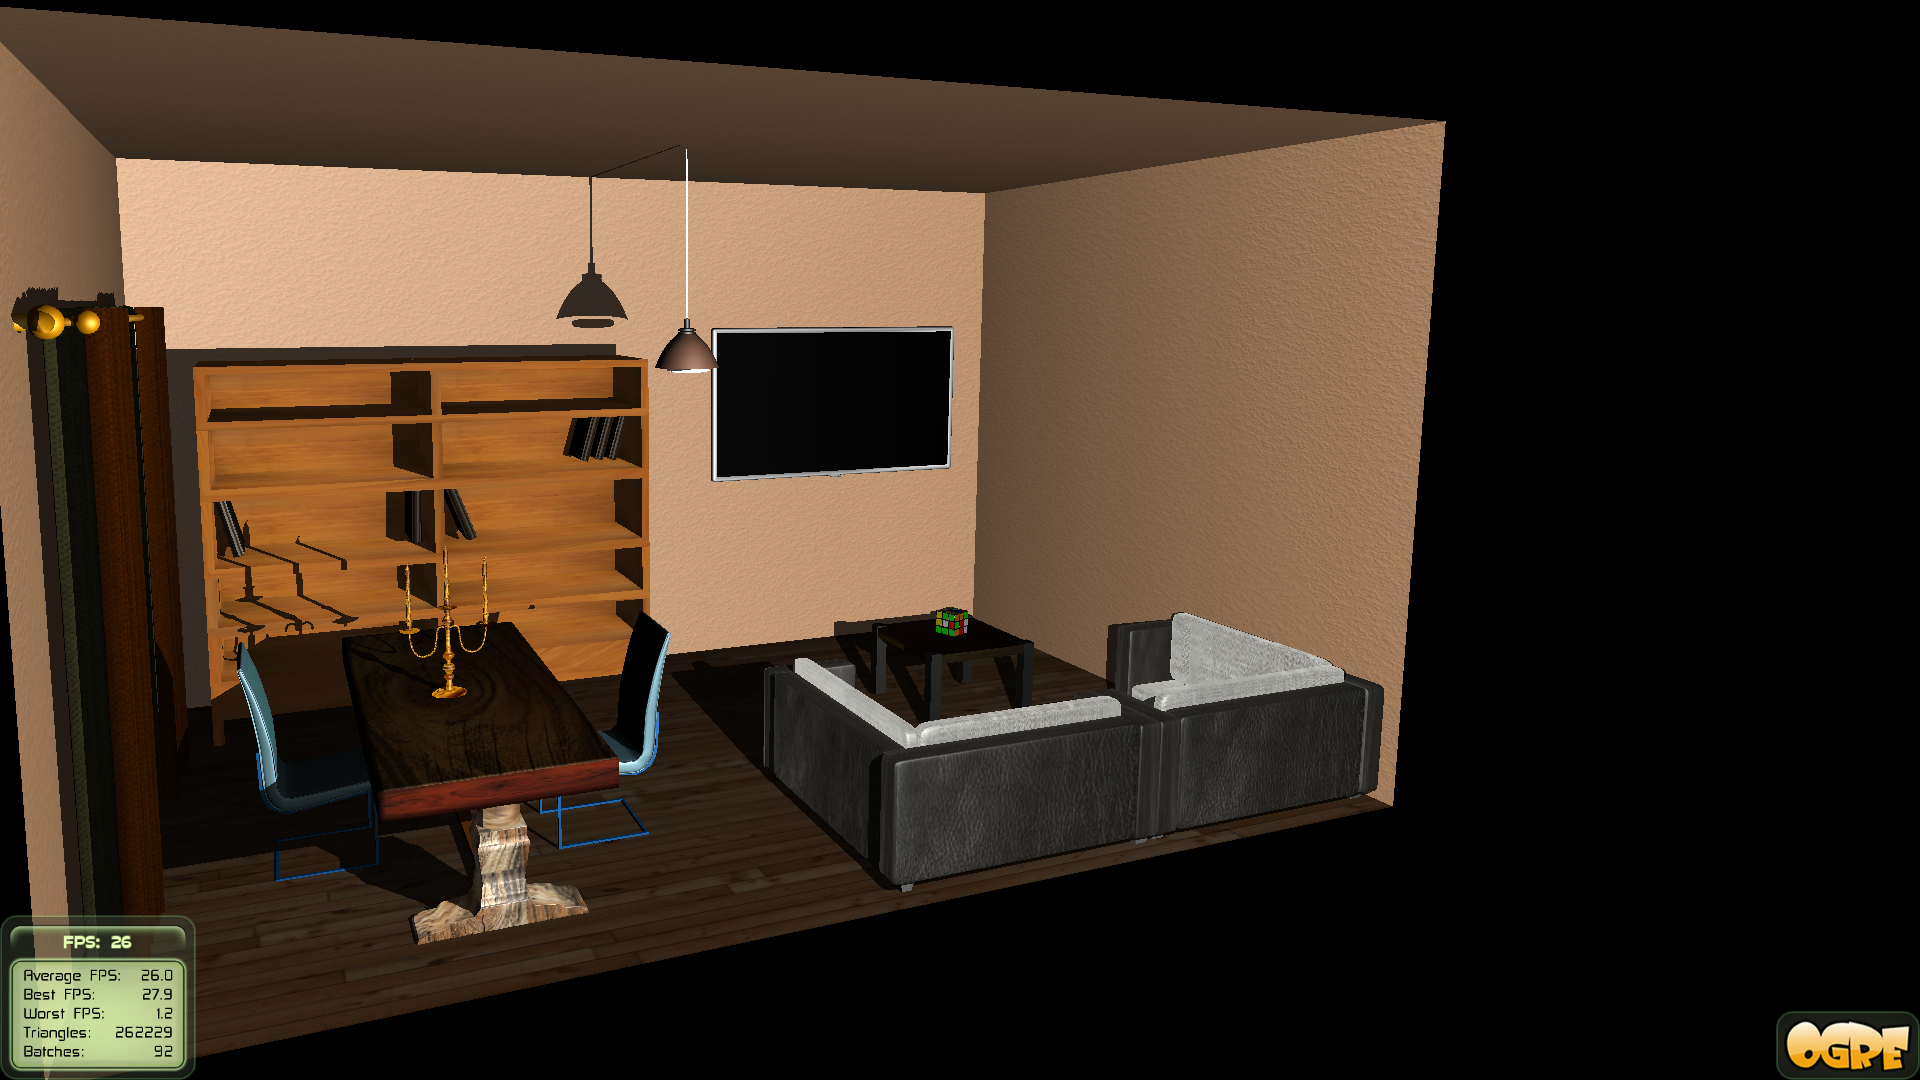
\includegraphics[width=0.7\textwidth]{images/progetto/ogre-wrong.png}
\caption{Trasformazione ottenuta calcolando in modo errato il vettore \textit{eye}.\label{wrong-eye}}
\end{figure}


\textit{target} è il centro del rettangolo che rappresenta il near plane, in quanto il punto osservato deve essere sempre il centro della scena.

In seguito viene richiamato un metodo che calcola la view matrix:

\begin{lstlisting}
Ogre::Vector3 up = Ogre::Vector3(0, 1, 0);
Ogre::Vector3 z = (eye - target); 
z.normalise();     // forward vector.
Ogre::Vector3 x = (up.crossProduct(z)); 
x.normalise();    // right vector.
Ogre::Vector3 y = z.crossProduct(x); // up vector.
 
Ogre::Matrix4 viewMatrix = Ogre::Matrix4(
    x.x, x.y, x.z, -(x.dotProduct(eye)),
    y.x, y.y, y.z, -(y.dotProduct(eye)),
    z.x, z.y, z.z, -(z.dotProduct(eye)),
      0,   0,   0,                    1
);
\end{lstlisting}
Il vettore \textit{up} equivale all'asse Y; la base ortonormale e la matrice sono calcolati come è stato visto nella sezione relativa alle trasformazioni.


\subsection*{Step 6: Traslazione} 
Grazie alle trasformazioni calcolate in precedenza, la prospettiva della telecamera virtuale viene collegata a quella dell'utente; tuttavia sono generati anche degli spostamenti indesiderati della scena, che possono farla scomparire oltre lo schermo, in quanto la telecamera virtuale in realtà sta fluttuando in base ai nostri movimenti. La figura \ref{no-transl} mostra l'effetto indesiderato.

\begin{figure}[htbp]
\centering
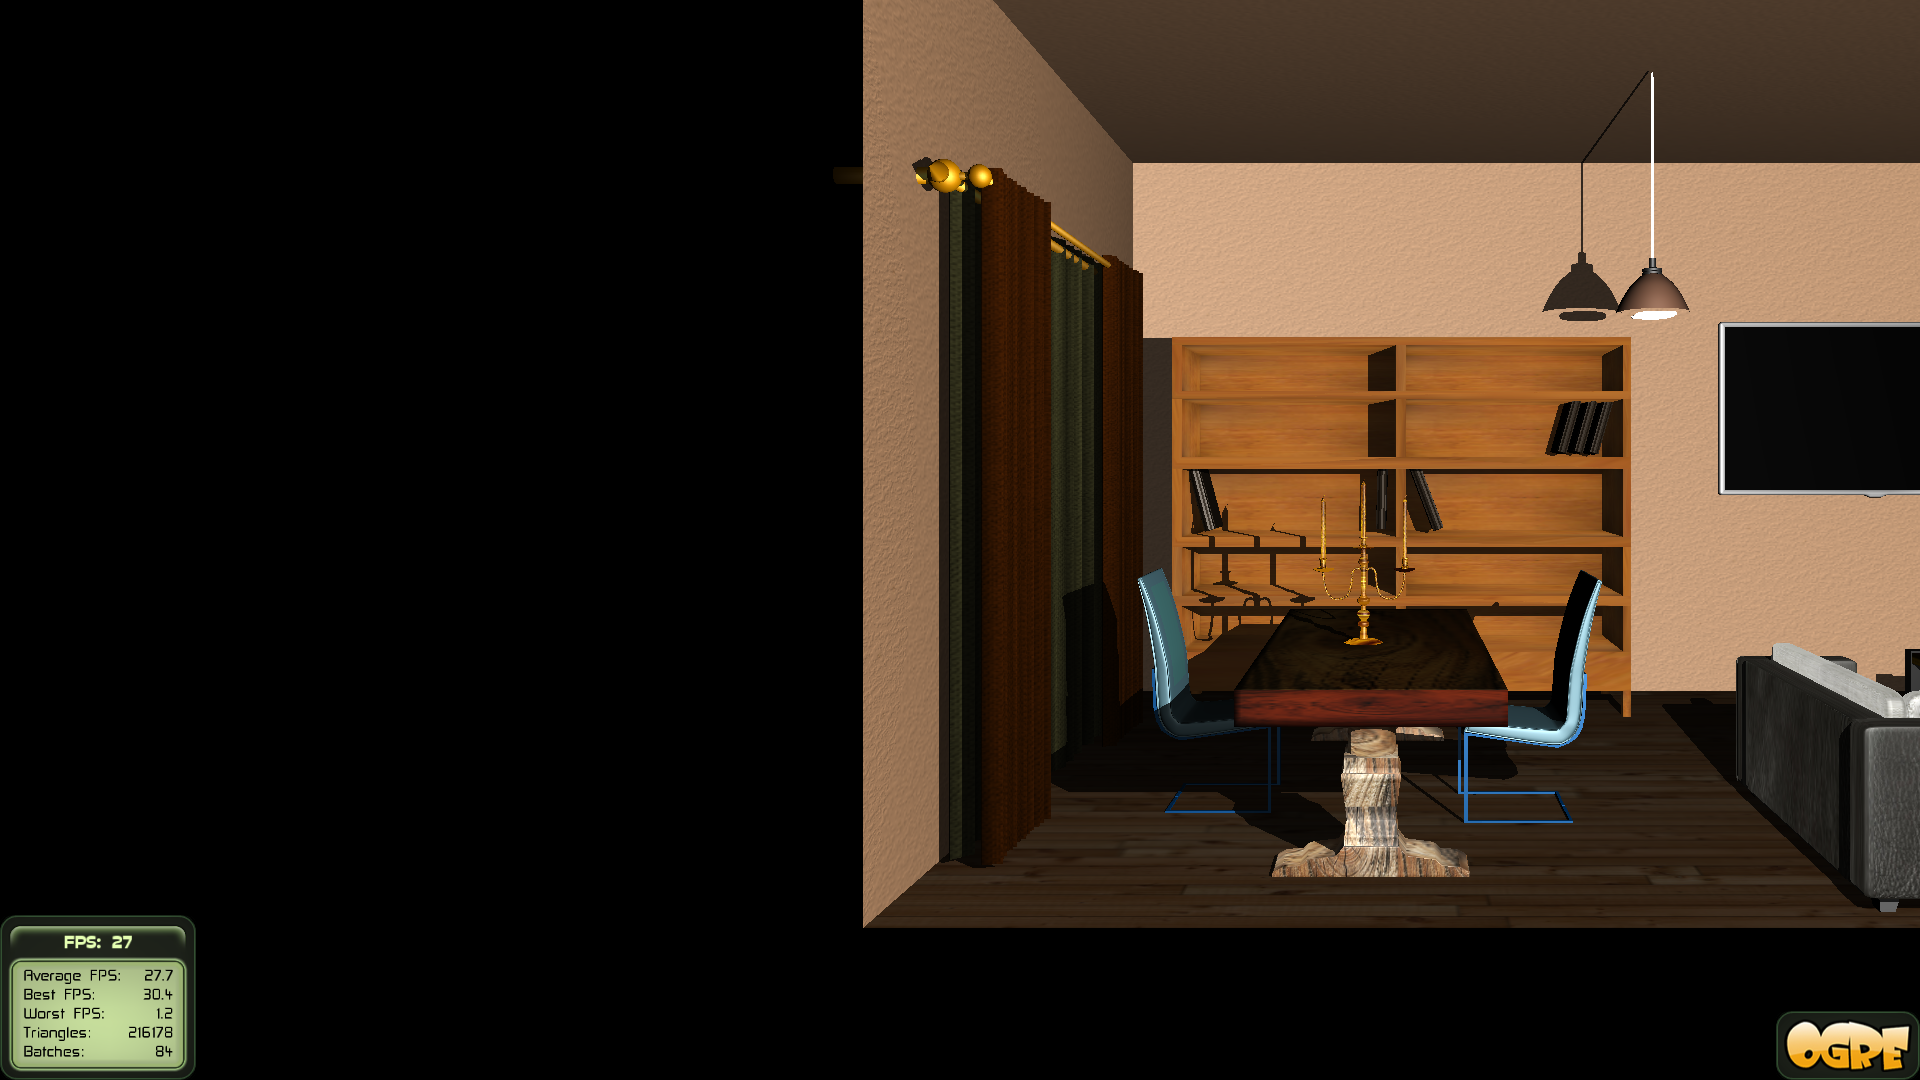
\includegraphics[width=0.7\textwidth]{images/progetto/ogre-transl.png}
\caption{Scena fluttuante, dovuta all'assenza di traslazione.\label{no-transl}}
\end{figure}
Per ottenere un corretto risultato, la scena deve rimanere ferma, cioè l'apertura della scatola deve essere fissata allo schermo; per ottenere ciò occorre una traslazione che annulli gli spostamenti generati.
\vspace{1.5cm}

\begin{lstlisting}
Ogre::Vector3 translVec = Ogre::Vector3(
            -face.x + r - width,
            -face.y + t - height,
            0
    );

Ogre::Matrix4 translMat = Ogre::Matrix4::IDENTITY;
translMat.makeTrans(translVec);
\end{lstlisting}
Si calcola il vettore \textit{translVec}, che rappresenta lo spostamento da effettuare, e poi questo viene passato come parametro al metodo \texttt{makeTrans}, il quale restituisce la matrice di traslazione desiderata.

\subsection*{Step 7: Trasformazione finale}
In OpenGL la trasformazione finale, relativa alla telecamera, è rappresentata da una matrice, che è il prodotto tra la traslazione, la matrice di proiezione e la view matrix:
\vspace{0.5cm}
\begin{lstlisting}
camera = translMat * frustum * viewMatrix;
\end{lstlisting}
In Ogre questa operazione è eseguita dal framework, perciò è sufficiente impostare le matrici calcolate, richiamando i seguenti metodi:
\begin{lstlisting}
mCamera->setCustomViewMatrix(true, translMat*viewMatrix);
mCamera->setCustomProjectionMatrix(true,frustum);
\end{lstlisting}



\section{Importazione scene}
Un'ulteriore feature dell'applicazione è quella di poter importare dall'esterno una qualsiasi scena, per poterla visualizzare in modo più interattivo.

%Un'ulteriore feature che si voleva aggiungere all'applicazione era quella di poter caricare una qualsiasi scena, modellata con diversi software, per poterla visualizzare in modo più interattivo.

\subsection{Importazione con OpenGL}
In OpenGL è stato utilizzato un parser per file con estensione .obj\footnote{File esportati da Blender, che contengono informazioni quali le coordinate dei vertici, delle normali, coordinate uv per mappare le texture, etc..}, il quale inserisce le informazioni dei modelli nei buffer utilizzati per il rendering. All'avvio del programma viene esaminata una directory apposita e, per ogni file .obj rilevato, ne viene fatto il parsing. In questo modo, per ogni modello, vengono creati diversi buffer, che saranno usati nella fase di rendering.

Purtroppo questo processo si è rivelato oneroso in OpenGL e ha portato anche ad alcune problematiche che hanno determinato la scelta di compiere questo ulteriore passo utilizzando il framework Ogre3D.

\subsection{Importazione con Ogre3D}
Esistono diversi exporter per software di modellazione quali Blender, Maya, 3D Studio Max, etc, per esportare scene e convertirle nel formato riconosciuto da Ogre. I modelli hanno estensione .mesh, mentre le informazioni relative ai materiali sono raccolte in file con estensione .material.

Per ottenere effetti più apprezzabili nelle trasformazioni, conviene che la scena rappresentata sia racchiusa da un box, con l'apertura frontale. Come esempio è stata preparata una scena in Blender, raffigurante un salotto, come si può vedere nella figura \ref{liv-room} \footnote{Alcuni modelli sono stati scaricati dal sito BlendSwap\cite{blendswap}.}.

\begin{figure}[htbp]
\centering
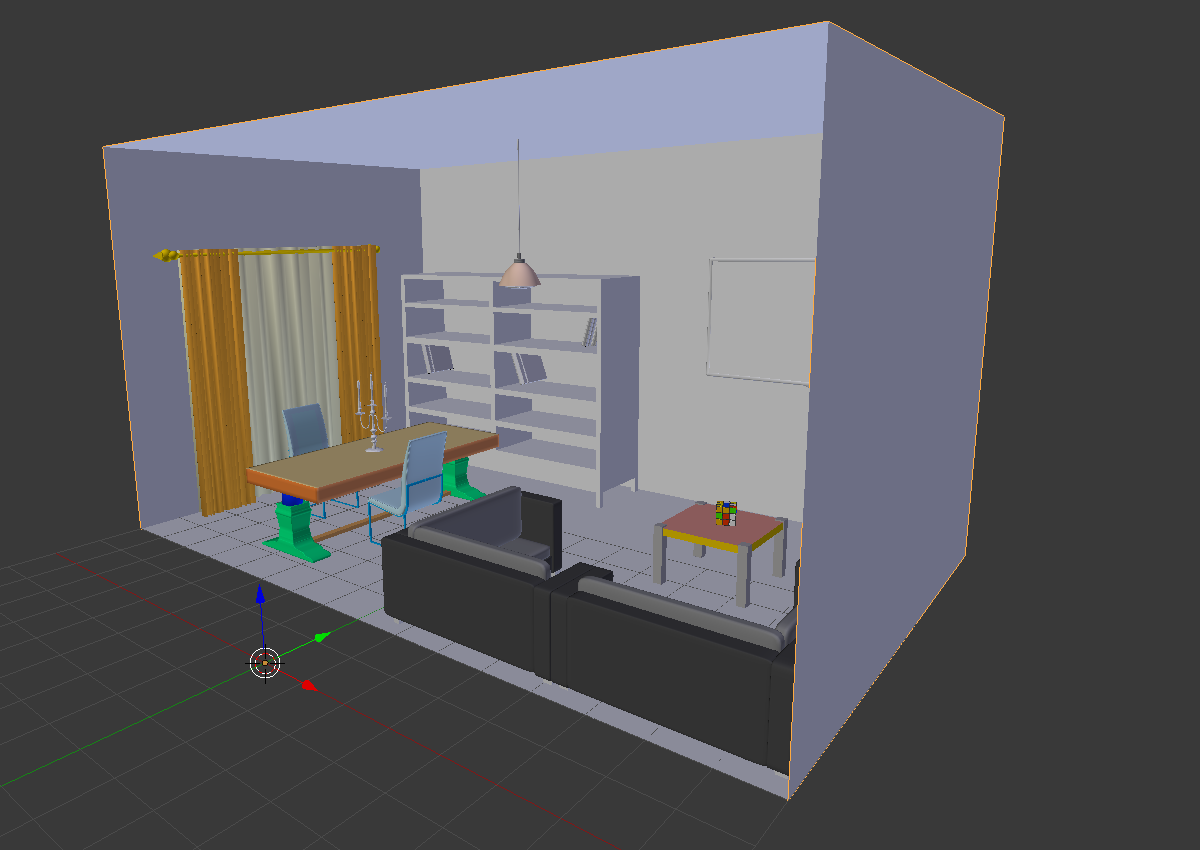
\includegraphics[width=0.7\textwidth]{images/progetto/living-room.png}
\caption{Scena modellata in Blender.\label{liv-room}}
\end{figure}

Da notare il fatto che le misure del box che racchiude la scena, in questo caso, ha un aspect ratio di $16/9$, infatti la lunghezza è pari a 16 unità mentre l'altezza è di 9 unità. Sono state scelte queste dimensioni per rispettare l'aspect ratio dello schermo. In Ogre è possibile scegliere la risoluzione della finestra all'avvio dell'applicazione, perciò si deve fare attenzione a rispettare il formato, in quanto rapporti diversi possono creare effetti di stiramento o di rimpicciolimento lungo una o entrambe le dimensioni.

Per ottenere una trasformazione corretta, il nostro frustum dovrebbe avere le stesse dimensioni della scena importata, ed inoltre il near plane andrebbe posizionato ad una distanza pari alla distanza da dove inizia la scena, in modo che il near plane coincida con l'apertura del box.

Un'ulteriore operazione da fare, all'avvio dell'applicazione, è quella di traslare la scena in modo che sia centrata nell'origine, per rientrare nella porzione di spazio considerato nel frustum.
Dopo la traslazione la scena sarà posta come è visibile nella figura \ref{transl-liv-room}. L'origine è rappresentato dai tre assi cartesiani colorati.

\begin{figure}[htbp]
\centering
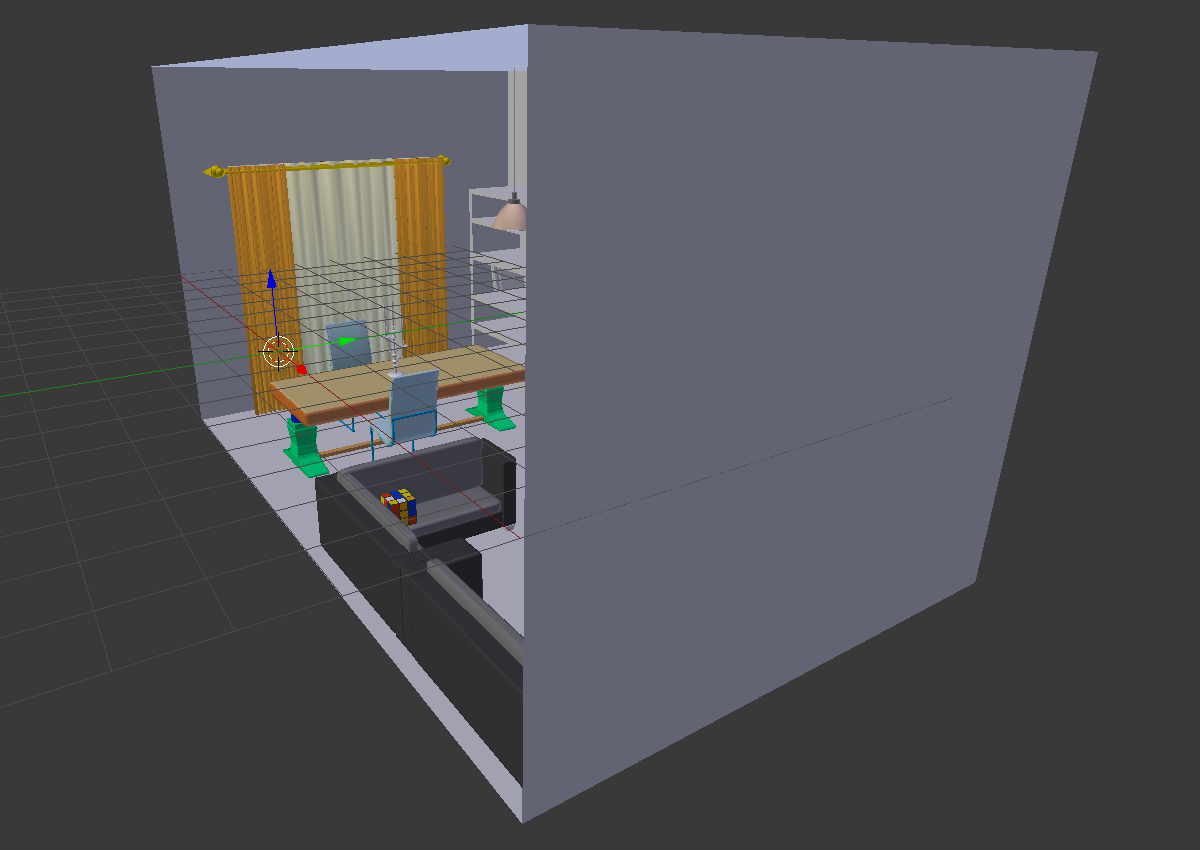
\includegraphics[width=0.7\textwidth]{images/progetto/living-room-translated.png}
\caption{La scena dopo la traslazione.\label{transl-liv-room}}
\end{figure}


Per quanto riguarda la $z$, la nostra scena inizia alla coordinata $y=2$ (l'asse Y di Blender corrisponde all'asse -Z in Ogre3D), perciò il near plane sarà posto ad una distanza pari a 2 lungo l'asse -Z, rispetto all'origine. Ovviamente il near plane è variabile, per determinare gli effetti di allontanamento o avvicinamento, ma comunque lo spostamento è corretto dalla view matrix, in modo che il near plane sia sempre coincidente con l'apertura del box.

Tutte queste condizioni sono necessarie affinché i bordi della scena siano sempre fissati ai bordi dello schermo del pc, in modo da illudere maggiormente l'occhio. Ovviamente senza questi accorgimenti la trasformazione continuerebbe comunque a funzionare in modo corretto, ma gli effetti ottenuti non garantirebbero l'illusione che l'applicazione ha lo scopo di creare.
 





\chapter{Risultati e discussioni}
\fancyhead[RO]{\bfseries Risultati e discussioni}

\section{Difficoltà e problematiche riscontrate}

Nello sviluppo del progetto sono state riscontrate varie problematiche, dovute anche ai limiti del software e dell'hardware utilizzato.


\subsection{Lo studio delle trasformazioni}
Lo studio per formulare il metodo usato per creare le giuste trasformazioni, ha occupato diverse giornate di lavoro, all'incirca una trentina. Questo soprattutto perchè la computer grafica, quando si tratta di teoria matematica, non è sempre facilmente comprensibile.

Infatti, dopo aver studiato le basi delle trasformazioni, trattate anche in questa tesi, esse sono state sviluppate procedendo sia per ragionamenti dovuti a calcoli preliminari, sia per tentativi puramente casuali. Fare prove inserendo valori casuali nelle varie operazioni è stato d'aiuto, in effetti, per comprendere meglio le variazioni del comportamento del sistema. Una volta trovata la trasformazione corretta, tuttavia, il procedimento ancora non era ben chiaro, perciò si è continuato a fare ulteriori prove. Tutto ciò è stato utile a comprendere quando la trasformazione funzionasse, o meglio, a stabilire le condizioni necessarie per produrre l'effetto desiderato e quindi rendere la trasformazione efficacie.



\subsection{I limiti dell'hardware}
L'obiettivo del progetto era quello di creare un'applicazione usufruibile da ogni utente, disponendo solamente di un pc e una webcam. Tuttavia si è notato che la qualità dell'hardware incide nella resa dell'applicazione.

Le prime prove erano fatte utilizzando le coordinate del mouse, al posto delle coordinate del volto rilevato. Si è notato che, importando il modulo OpenCv, la velocità di esecuzione veniva fortemente rallentata, perchè il solo rilevamento è un processo molto dispendioso. Aggiungengo il carico di lavoro dovuto alla parte grafica, il risultato era inaccettabile, renderizzando circa 15 frames al secondo (utilizzando un processore Intel I5 e una scheda grafica ATI Radeon HD 5650, quindi hardware di qualità medio-alta).

Fortunatamente esisteva un parametro, nella funzione \textit{detect\_multi\_scale()} situato nel modulo OpenCv, che ha permesso di migliorare la velocità senza diminuire la qualità. Questo parametro era relativo alle dimensioni dell'area minima da analizzare per il rilevamento; più è piccola l'area e più calcoli deve eseguire l'algoritmo per riconoscere i volti. All'inizio era impostato a $(30,30)$, in questo modo i volti venivano ricercati in aree di minimo 30 pixel per 30. Aumentanto questo valore a circa $(100,100)$, la velocità di esecuzione è stata portata a 30 frames al secondo, utilizzando anche scene complesse, in cui erano presenti alcune centinaia di migliaia di vertici. Questi valori permettono, in una webcam di risoluzione $640\times480$, di rilevare volti fino ad una distanza di circa un metro e mezzo dallo schermo, perciò il compromesso è accettabile.

La qualità della webcam può incidere nel miglioramento della qualità, potendo diminuire il rumore generato dall'imprecisione del rilevamento. Tuttavia, aumentare la risoluzione della webcam potrebbe incidere nella velocità, per il motivo precedente, ovvero perchè i frames che OpenCv deve analizzare, hanno dimensioni più elevate, perciò deve effettuare più calcoli.

Allo stesso modo può influire l'angolo di apertura della webcam: più è elevato e meglio si può apprezzare l'illusione, in quanto l'utente ha più spazio per potersi muovere senza essere perso dall'obiettivo della webcam, generando interruzioni nella trasformazione. 

\subsection{I limiti di OpenCv}

Come è stato già accennato, OpenCv fornisce dei metodi che hanno delle limitazioni: il rilevamento non è preciso, generando sempre una sorta di oscillamento nelle coordinate rilevate durante il tracking, e non è in grado di stimare la distanza dallo schermo.

Per quanto riguarda il primo limite si può dire che, grazie all'aggiunta dell'algoritmo che funge da filtro, il problema è stato risolto senza incidere troppo sulla qualità finale.

Per quanto riguarda il secondo limite invece non è stato raggiunto il risultato sperato. Per un effetto più realistico infatti, la trasformazione dovrebbe tenere conto in modo preciso della distanza dell'utente, perchè le coordinate x e y andrebbero calcolate in funzione anche di essa.

Questo perchè anche la webcam possiede un proprio frustum, e quindi spostamenti lungo l'asse x o y non rimangono proporzionati al variare della distanza, ovvero la coordinata z. Infatti, all'aumentare della distanza dallo schermo, gli spostamenti rilevati lungo gli assi x e y variano più lentamente, di conseguenza la prospettiva sarà trasformata più lentamente.

Il calcolo della distanza non è banale con una semplice webcam. Bisognerebbe effettuare una calibrazione ad ogni esecuzione per misurare la grandezza della testa dell'utente in modo da trovare un coefficiente per ricalcolare la x e la y. Poichè anche il rilevamento non è preciso e varia in base a molti fattori, questa caratteristica richiede uno studio molto approfondito, e un gran numero di prove.

Il problema potrebbe essere risolto utilizzando un sensore apposito, come il Kinect della Microsoft, che stima in modo abbastanza preciso le distanze grazie a raggi infrarossi, ma questo andrebbe contro la logica dell'applicazione, che mira ad offrire questa forma di interazione utilizzando semplicemente una webcam.

\subsection{Importazione modelli in OpenGL}
In OpenGl è stato riscontrato un problema nell'importazione dei modelli 3D con estensione .obj. Infatti quando erano renderizzati a schermo, risultava che la trasformazione che essi subivano fosse ritardata di uno o due frames rispetto agli altri oggetti disegnati direttamente in OpenGL. Questo generava un'irregolarità nel movimento apparente degli oggetti, producendo un'effetto simile ad una sorta di tremolio.

Il difetto probabilmente era legato ai driver della scheda grafica, tuttavia non sono state fatte prove su altre macchine quindi il problema è rimasto irrisolto.

Successivamente lo sviluppo è passato ad Ogre3D, che permette di gestire più efficientemente scene importate dall'esterno, perciò la parte OpenGL è stata messa da parte. Con Ogre3D il problema non è ricomparso.



\section{I requisiti dell'applicazione}
In questo paragrafo riassumiamo le condizioni che devono essere rispettate per la miglior resa dell'applicazione:
\begin{itemize}
\item \textit{Ambiente}: L'ambiente in cui si usa l'applicazione deve essere ben illuminato, per riconoscere meglio i volti. La scarsa illuminazione rende anche più faticoso il rilevamento, causando una caduta di prestazioni in termini di velocità di esecuzione.

Inoltre lo spazio intorno all'utente dovrebbe essere libero da cose che possono creare interferenze o falsi positivi (altre persone, magliette, disegni o poster raffiguranti volti, etc).

\item \textit{Webcam}: La webcam dovrebbe essere di buona qualità, ma con una risoluzione non troppo alta, per evitare che le dimensioni dei frame rendano il rilevamento troppo complesso (questo se si utilizzano un processore e una scheda grafica di media potenza).

Inoltre la webcam deve essere posizionata sopra lo schermo, al centro, cioè nella posizione di default dei computer portatili. Se viene posizionata in altri punti, il volto rilevato renderebbe la prospettiva dell'utente non più allineata con quella della telecamera virtuale.

\item \textit{Scena 3D}: Per rendere l'illusione più efficiente (come già detto la trasformazione è corretta anche se la scena non rispetta queste condizioni), la scena 3D importata dovrebbe essere racchiusa in un box, le cui dimensioni dovrebbero essere uguali alle dimensioni del frustum, con l'apertura giaciente sul near plane. Inoltre l'aspect ratio del box dovrebbe rispettare quella dello schemo, per evitare stiramenti o rimpicciolimenti della scena.

Nel progetto sviluppato in Ogre3D è stato aggiunto un file di configurazione, dove l'utente può specificare le coordinate dei punti che identificano il suo box. Tramite queste coordinate il programma imposta le dimensioni del frustum e trasla la scena centrandola nell'origine, allineandola così con il frustum. 

Grazie a queste accortezze l'apertura del box rimane coincidente con lo schermo (se si usa lo schermo intero), e, durante la trasformazione di prospettiva, i bordi rimangono allineati, creando l'illusione che la scatola abbia profondità.
\end{itemize}

\section{Risultati}
Nel corso dello sviluppo del progetto sono stati apportati notevoli miglioramenti nel funzionamento dell'applicazione. Essa è stata provata da alcuni utenti (familiari e conoscenti), e tutti sono rimasti affascinati dall'effetto prodotto. Arrivati al punto attuale, perciò, si può dire che i risultati sono accettabili, in quanto l'illusione che si vuole creare è più che apprezzabile.



\addcontentsline{toc}{chapter}{Conclusioni}
\fancyhead[RO]{\bfseries Conclusioni}

\chapter*{Conclusioni}
In questa tesi è stata trattata un'applicazione che presenta un'interfaccia uomo-macchina per l'interazione con un sistema virtuale. In particolare essa trasforma lo stesso utente nel controller del sistema visivo per una scena virtuale. La prospettiva con cui è vista la scena è trasformata in funzione delle coordinate del volto rilevato. L'obiettivo è creare l'illusione che ci sia profondità all'interno dello schermo, generando un effetto 3D.

L'applicazione è stata sviluppata utilizzando software completamente open-source. Sono stati usati:
OpenCv per il rilevamento del volto, OpenGL per lo studio della trasformazione adottata, Ogre3D per il miglioramento della resa della scena. Inoltre per la modellazione 3D si è usato Blender.

L'applicazione offre un'ulteriore feature, ovvero la possibilità di importare modelli dall'esterno. Esistono exporter che permettono di esportare scene modellate con diversi software, nel formato riconosciuto da Ogre3D. Tuttavia per ora si è preso in considerazione solamente l'exporter di Blender, perciò il funzionamento è garantito solo per scene esportate con questo software.

Richiedendo solamente un pc e una webcam, il programma è accessibile da tutti, ma presenta dei limiti. Il limite che influisce maggiormente è l'assenza del calcolo preciso della distanza dell'utente dallo schermo. Questo problema rende non uniformi gli spostamenti dell'utente, se si trova a distanze differenti.

Al di là dei limiti, l'applicazione produce un effetto positivo, soprattutto nell'utente medio, magari non abituato ad illusioni di questo genere, perciò il risultato si può considerare più che accettabile.

L'applicazione presenta grandi potenzialità, potendo estendere il suo utilizzo per svariati scopi, a partire da semplice forma di intrattenimento, fino ad essere impiegato in simulazioni virtuali più complesse, come ad esempio i videogiochi. Il fatto che l'applicazione sia stata sviluppata con software open-source la rende completamente aperta a miglioramenti e sviluppi futuri. 


\newpage 
\addcontentsline{toc}{chapter}{Bibliografia}
\begin{thebibliography}{10}

\bibitem{vella2011gpu}
Vella, F., Cefal\`a, R., Costantini, A., Gervasi, O., Tanci, C.: Gpu computing
  in egi environment using a cloud approach. In: 2011 International Conference
  on Computational Science and Its Applications. pp. 150--155. IEEE (2011)
  
\bibitem{intro}
intro
%immagini
%http://upload.wikimedia.org/wikipedia/commons/f/fe/KinectSensor.png
%http://www.marcosiino.it/wp-content/uploads/2013/11/Oculus-Rift-1.jpg
%http://upload.wikimedia.org/wikipedia/commons/7/7d/Wiimote-Safety-First.jpg

\bibitem{realta}
realta
%%http://it.wikipedia.org/wiki/Realt\%C3\%A0\_virtuale\\
%%http://www.treccani.it/enciclopedia/realta-virtuale\_(Enciclopedia\_Italiana)/
%
\bibitem{opencv}
opencv
%
%http://it.wikipedia.org/wiki/Visione\_artificiale\\
%http://opencv.org/\\
%http://en.wikipedia.org/wiki/OpenCV\\
%http://it.wikipedia.org/wiki/Riconoscimento\_facciale\\
%http://it.wikipedia.org/wiki/Wavelet\_Haar\\
%http://it.wikipedia.org/wiki/Wavelet\_Haar\\
%http://docs.opencv.org/modules/contrib/doc/facerec/facerec\_tutorial.html\\
%http://docs.opencv.org/trunk/doc/py\_tutorials/py\_objdetect/py\_face\_detection/py\_face\_detection.html\\
%
%immagini\\
%\ref{features}\\
%%http://docs.opencv.org/trunk/_images/haar_features.jpg
%\ref{volti}\\
%%http://docs.opencv.org/trunk/_images/haar.png

\bibitem{opengl}

opengl
%http://it.wikipedia.org/wiki/OpenGL\\
%http://www.opengl.org/\\

\bibitem{ogre}
ogre
%http://www.ogre3d.org/\\
%http://en.wikipedia.org/wiki/OGRE\\
%http://www.stevestreeting.com/


\bibitem{frustum}
frustum


%fonti\\
%http://people.cs.clemson.edu/~dhouse/courses/817/notes/OpenGL-pipeline.pdf\\
%http://www.cse.ohio-state.edu/~whmin/courses/cse5542-2013-spring/10-transformation.pdf\\
%http://www.songho.ca/opengl/gl\_transform.html\\
%http://www.songho.ca/math/homogeneous/homogeneous.html
%http://3dgep.com/?p=1700\#Transformations\\
%libro: 3d math for game programming\\
%http://www.opengl-tutorial.org/beginners-tutorials/tutorial-3-matrices/\\
%
%immagini\\
%
%\ref{cam-default}\\ %http://www.google.it/imgres?imgurl=http%3A%2F%2Fschoolacademy.googlecode.com%2Fsvn%2Ftrunk%2FMeeting-9-3D-Studio-and-OpenGL-Immediate-Mode-Rendering%2Fimages%2Fopengl-camera-default.jpg&imgrefurl=http%3A%2F%2Fschoolacademy.googlecode.com%2Fsvn%2Ftrunk%2FMeeting-9-3D-Studio-and-OpenGL-Immediate-Mode-Rendering%2Fimages%2F&h=734&w=1024&tbnid=V0VT6QWQOnk6RM%3A&zoom=1&docid=TBEzNF1TZsRFsM&ei=o_dQU6f_HaLl4wSexoHwCg&tbm=isch&ved=0CFkQMygCMAI&iact=rc&uact=3&dur=3346&page=1&start=0&ndsp=28
%\ref{pipeline}\\
%%http://upload.wikimedia.org/wikipedia/commons/b/bb/Pipeline_OpenGL_(en).png
%\ref{trans-pipe}\\
%%http://www.songho.ca/opengl/files/gl_transform02.png
%\ref{cartesian}\\
%%http://lh6.ggpht.com/_QLwms0mVa4w/SeibBLR9xVI/AAAAAAAAARM/p_fKVgGsKm0/cartesian.png?imgmax=800
%\ref{view-frustum}\\
%%http://murlengine.com/tutorials/en/tut_01_01_view_frustum.png
%\ref{orto}\\
%%http://www.songho.ca/opengl/files/gl_projectionmatrix02.png
%\ref{persp}\\
%%http://www.songho.ca/opengl/files/gl_projectionmatrix01.png
%\ref{example1}\\
%%http://www.opengl-tutorial.org/wp-content/uploads/2011/04/nondeforme.png
%\ref{example2}\\
%%http://www.opengl-tutorial.org/wp-content/uploads/2011/04/homogeneous.png
%\ref{example3}\\
%%http://www.opengl-tutorial.org/wp-content/uploads/2011/04/projected1.png
%%http://stackoverflow.com/questions/17587752/setting-up-an-asymmetric-frustum
%



\bibitem{progetto}
progetto
%immagini\\
%salotto\\ %http://www.blendswap.com/blends/view/67465
%tv\\ %http://www.blendswap.com/blends/view/63306
%cubo\\%http://www.blendswap.com/blends/view/51422


\bibitem{risultati}
risultati

\bibitem{conclusioni}
conclusioni

\end{thebibliography}
     %conterra' una serie di istruzioni del tipo:    
                         % \bibitem{eol} O. Gervasi and A. Lagan‡ "EOL: A Web-Based Distance Assessment System", 
			 % Lecture Notes in Computer Science, 3044, Springer & Verlag, pp. 854-862 (2004)

%APPENDICE CON CODICE
%\appendix
%\linespread{1}
%\fancyhead[RO]{\bfseries Codice}
%\chapter*{Codice}
\section*{index.php}
\begin{footnotesize}
\begin{verbatim}
int x = 0;

for( int i = 0; i < x; i++ ) {
	std::cout << ciao << std::endl;
}

\end{verbatim}
\end{footnotesize}
%


\end{document}
